% ******************************* PhD Thesis Template **************************
% Please have a look at the README.md file for info on how to use the template


% \documentclass[a4paper,12pt,times,numbered,print,index,oneside]{Classes/PhDThesisPSnPDF}

%\documentclass[a4paper,12pt,Boisik,numbered,print,index,oneside]{Classes/PhDThesisPSnPDF}

\documentclass[a4paper,12pt,Palatino,numbered,print,index,oneside]{Classes/PhDThesisPSnPDF}

\usepackage{listings}
\usepackage{color}
\usepackage{shapepar}
\usepackage[T1]{fontenc}
\usepackage[utf8]{inputenc}
\usepackage{hyperref}
\usepackage{smartdiagram}

\definecolor{dkgreen}{rgb}{0,0.6,0}
\definecolor{gray}{rgb}{0.5,0.5,0.5}
\definecolor{mauve}{rgb}{0.58,0,0.82}
\definecolor{light-gray}{gray}{0.70}

\lstset{
%frame=none,
frame=single,
language=Python,
aboveskip=3mm,
belowskip=3mm,
showstringspaces=false,
columns=flexible,
basicstyle={\small\ttfamily},
numbers=none,
numberstyle=\tiny\color{gray},
keywordstyle=\color{blue},
commentstyle=\color{dkgreen},
stringstyle=\color{mauve},
breaklines=true,
breakatwhitespace=true,
tabsize=3
}

\usepackage{xcolor}

\usepackage{amsmath}
\usepackage{algorithm}

\usepackage[noend]{algpseudocode}
\algdef{SE}{Begin}{End}{\textbf{begin}}{\textbf{end}}

\usepackage{caption}

\usepackage{subfig}

\DeclareCaptionFont{white}{\color{white}}
\DeclareCaptionFormat{listing}{\colorbox{black}{\parbox{\textwidth}{#1#2#3}}}
\captionsetup[lstlisting]{format=listing,labelfont=white,textfont=white, margin=0pt}

% \usepackage{titlesec}
% \newcommand*{\justifyheading}{\raggedleft}
% \titleformat{\chapter}[display]
%   {\normalfont\huge\bfseries\justifyheading}{\chaptertitlename\ \thechapter}
%   {20pt}{\Huge}

% \usepackage{indentfirst}

% ******************************************************************************
% ******************************* Class Options ********************************
% *********************** See README for more details **************************
% ******************************************************************************

% `a4paper'(The University of Cambridge PhD thesis guidelines recommends a page
% size a4 - default option) or `a5paper': A5 Paper size is also allowed as per
% the Cambridge University Engineering Deparment guidelines for PhD thesis
%
% `11pt' or `12pt'(default): Font Size 10pt is NOT recommended by the University
% guidelines
%
% `oneside' or `twoside'(default): Printing double side (twoside) or single
% side.
%
% `print': Use `print' for print version with appropriate margins and page
% layout. Leaving the options field blank will activate Online version.
%
% `index': For index at the end of the thesis
%
% `draftclassic': For draft mode without loading any images (same as draft in book)
%
% `draft': Special draft mode with line numbers, images, and water mark with
% timestamp and custom text. Position of the text can also be modified.
%
% `abstract': To generate only the title page and abstract page with
% dissertation title and name, to submit to the Student Registry
%
% `chapter`: This option enables only the specified chapter and it's references
%  Useful for review and corrections.
%
% ************************* Custom Page Margins ********************************
%
% `custommargin`: Use `custommargin' in options to activate custom page margins,
% which can be defined in the preamble.tex. Custom margin will override
% print/online margin setup.
%
% *********************** Choosing the Fonts in Class Options ******************
%
% `times' : Times font with math support. (The Cambridge University guidelines
% recommend using times)
%
% `fourier': Utopia Font with Fourier Math font (Font has to be installed)
%            It's a free font.
%
% `customfont': Use `customfont' option in the document class and load the
% package in the preamble.tex
%
% default or leave empty: `Latin Modern' font will be loaded.
%
% ********************** Choosing the Bibliography style ***********************
%
% `authoryear': For author-year citation eg., Krishna (2013)
%
% `numbered': (Default Option) For numbered and sorted citation e.g., [1,5,2]
%
% `custombib': Define your own bibliography style in the `preamble.tex' file.
%              `\RequirePackage[square, sort, numbers, authoryear]{natbib}'.
%              This can be also used to load biblatex instead of natbib
%              (See Preamble)
%
% **************************** Choosing the Page Style *************************
%
% `default (leave empty)': For Page Numbers in Header (Left Even, Right Odd) and
% Chapter Name in Header (Right Even) and Section Name (Left Odd). Blank Footer.
%
% `PageStyleI': Chapter Name next & Page Number on Even Side (Left Even).
% Section Name & Page Number in Header on Odd Side (Right Odd). Footer is empty.
%
% `PageStyleII': Chapter Name on Even Side (Left Even) in Header. Section Number
% and Section Name in Header on Odd Side (Right Odd). Page numbering in footer

% Uncomment to change page style
%\pagestyle{PageStyleII}

% ********************************** Preamble **********************************
% Preamble: Contains packages and user-defined commands and settings
% ******************************************************************************
% ****************************** Custom Margin *********************************
\usepackage[italian,english]{babel}

% Add `custommargin' in the document class options to use this section
% Set {innerside margin / outerside margin / topmargin / bottom margin}  and
% other page dimensions
\ifsetCustomMargin
  \RequirePackage[left=37mm,right=30mm,top=35mm,bottom=30mm]{geometry}
  \setFancyHdr % To apply fancy header after geometry package is loaded
\fi

% Add spaces between paragraphs
%\setlength{\parskip}{0.5em}
% Ragged bottom avoids extra whitespaces between paragraphs
\raggedbottom
% To remove the excess top spacing for enumeration, list and description
%\usepackage{enumitem}
%\setlist[enumerate,itemize,description]{topsep=0em}

% *****************************************************************************
% ******************* Fonts (like different typewriter fonts etc.)*************

% Add `customfont' in the document class option to use this section

\ifsetCustomFont
  % Set your custom font here and use `customfont' in options. Leave empty to
  % load computer modern font (default LaTeX font).
  %\RequirePackage{helvet}

  % For use with XeLaTeX
  %  \setmainfont[
  %    Path              = ./libertine/opentype/,
  %    Extension         = .otf,
  %    UprightFont = LinLibertine_R,
  %    BoldFont = LinLibertine_RZ, % Linux Libertine O Regular Semibold
  %    ItalicFont = LinLibertine_RI,
  %    BoldItalicFont = LinLibertine_RZI, % Linux Libertine O Regular Semibold Italic
  %  ]
  %  {libertine}
  %  % load font from system font
  %  \newfontfamily\libertinesystemfont{Linux Libertine O}
\fi

% *****************************************************************************
% **************************** Custom Packages ********************************

% ************************* Algorithms and Pseudocode **************************

%\usepackage{algpseudocode}


% ********************Captions and Hyperreferencing / URL **********************

% Captions: This makes captions of figures use a boldfaced small font.
%\RequirePackage[small,bf]{caption}

\RequirePackage[labelsep=space,tableposition=top]{caption}
\renewcommand{\figurename}{Fig.} %to support older versions of captions.sty


% *************************** Graphics and figures *****************************

%\usepackage{rotating}
%\usepackage{wrapfig}

% Uncomment the following two lines to force Latex to place the figure.
% Use [H] when including graphics. Note 'H' instead of 'h'
%\usepackage{float}
%\restylefloat{figure}

% Subcaption package is also available in the sty folder you can use that by
% uncommenting the following line
% This is for people stuck with older versions of texlive
%\usepackage{sty/caption/subcaption}
% \usepackage{subcaption}

% ********************************** Tables ************************************
\usepackage{booktabs} % For professional looking tables
\usepackage{multirow}

%\usepackage{multicol}
%\usepackage{longtable}
%\usepackage{tabularx}


% *********************************** SI Units *********************************
\usepackage{siunitx} % use this package module for SI units


% ******************************* Line Spacing *********************************

% Choose linespacing as appropriate. Default is one-half line spacing as per the
% University guidelines

% \doublespacing
\onehalfspacing
% \singlespacing


% ************************ Formatting / Footnote *******************************

% Don't break enumeration (etc.) across pages in an ugly manner (default 10000)
%\clubpenalty=500
%\widowpenalty=500

%\usepackage[perpage]{footmisc} %Range of footnote options


% *****************************************************************************
% *************************** Bibliography  and References ********************

%\usepackage{cleveref} %Referencing without need to explicitly state fig /table

% Add `custombib' in the document class option to use this section
\ifuseCustomBib
   \RequirePackage[square, sort, numbers, authoryear]{natbib} % CustomBib

% If you would like to use biblatex for your reference management, as opposed to the default `natbibpackage` pass the option `custombib` in the document class. Comment out the previous line to make sure you don't load the natbib package. Uncomment the following lines and specify the location of references.bib file

% \RequirePackage[backend=biber, style=numeric-comp, citestyle=numeric, sorting=nty, natbib=true]{biblatex}
% \bibliography{References/references} %Location of references.bib only for biblatex

\fi

% changes the default name `Bibliography` -> `References'
\renewcommand{\bibname}{References}


% ******************************************************************************
% ************************* User Defined Commands ******************************
% ******************************************************************************

% *********** To change the name of Table of Contents / LOF and LOT ************

%\renewcommand{\contentsname}{My Table of Contents}
%\renewcommand{\listfigurename}{My List of Figures}
%\renewcommand{\listtablename}{My List of Tables}


% ********************** TOC depth and numbering depth *************************

\setcounter{secnumdepth}{2}
\setcounter{tocdepth}{2}


% ******************************* Nomenclature *********************************

% To change the name of the Nomenclature section, uncomment the following line

%\renewcommand{\nomname}{Symbols}


% ********************************* Appendix ***********************************

% The default value of both \appendixtocname and \appendixpagename is `Appendices'. These names can all be changed via:

%\renewcommand{\appendixtocname}{List of appendices}
%\renewcommand{\appendixname}{Appndx}

% *********************** Configure Draft Mode **********************************

% Uncomment to disable figures in `draft'
%\setkeys{Gin}{draft=true}  % set draft to false to enable figures in `draft'

% These options are active only during the draft mode
% Default text is "Draft"
%\SetDraftText{DRAFT}

% Default Watermark location is top. Location (top/bottom)
%\SetDraftWMPosition{bottom}

% Draft Version - default is v1.0
%\SetDraftVersion{v1.1}

% Draft Text grayscale value (should be between 0-black and 1-white)
% Default value is 0.75
%\SetDraftGrayScale{0.8}


% ******************************** Todo Notes **********************************
%% Uncomment the following lines to have todonotes.

%\ifsetDraft
%	\usepackage[colorinlistoftodos]{todonotes}
%	\newcommand{\mynote}[1]{\todo[author=kks32,size=\small,inline,color=green!40]{#1}}
%\else
%	\newcommand{\mynote}[1]{}
%	\newcommand{\listoftodos}{}
%\fi


% \titleformat{\chapter}[chapter]{\filleft\Huge\bfseries}{\thechapter\hsp\textcolor{gray75}{|}\hsp}{0pt}{\Huge\bfseries}
\pagenumbering{roman}
\begin{document}
\selectlanguage{italian}

% ************************ Thesis Information & Meta-data **********************
% Thesis title and author information, refernce file for biblatex
\begin{titlepage}
\begin{center}


{\large Università degli Studi di Salerno}\\[0.2truecm]
{\large Dipartimento di Informatica}\\

% \vfill

\begin{figure}[htbp]
\centering

\includegraphics[height=3cm, width=3cm]{Figure/logounisa.png}
\end{figure}

% \vfill

{\large Corso di Laurea in Informatica}

\vfill\vfill

{\Huge \textbf{TiveJS}}

\vspace{0.2cm}

{\LARGE Un'applicazione Javascript per il riconoscimento di linguaggi diagrammatici} 
\newline \newline
{\LARGE A Javascript application for the recognition of Diagrammatic languages}

\vfill\vfill

{\bf Relatori}              \hfill {\bf Candidato}  \\
Prof. Gennaro Costagliola   \hfill Dario Tecchia  \\
Dott. Mattia De Rosa        \hfill Matr. 0512102581 \\

\vfill
\hrulefill 

Anno Accademico 2018/2019

\end{center}
\end{titlepage}

% ***************************** Abstract Separate ******************************

\ifdefineAbstract
    \includeonly{Abstract/abstract}
\fi

% ******************************** Front Matter ********************************

\begin{dedication}

\begin{flushright}

\textit{Questa tesi la dedico alla mia famiglia.}

\end{flushright}

\end{dedication}

\newpage

\chapter*{Ringraziamenti}
\addcontentsline{toc}{chapter}{Ringraziamenti}

\newpage

\chapter*{Abstract}
\addcontentsline{toc}{chapter}{Abstract}

    La comunicazione visiva è in molti casi più diretta ed immediata rispetto alla comunicazione verbale: disegni, foto e mappe sono esempi di frasi visive che necessitano di un contesto per essere descritte in modo naturale.
    \newline
    In questa tesi presento TiveJS, un'estensione della piattaforma \href{https://www.draw.io/}{draw.io}, che sfrutta  simboli e  definizioni sematiche per il riconoscimento dei linguaggi diagrammatici e la traduzione di questi in altri linguaggi.
    Il tool applica  delle definizioni semantiche  ad un diagramma e restituisce una traduzione di quest'ultimo. La traduzione avviene attraverso due fasi principali: il riconoscimento del grafo e l'applicazione delle definizioni.
    \newline
    Il mio lavoro di tesi si basa su strumenti precedentemente sviluppati: LoCoModeler e Tive. Precedentemente suddiviso in lato client e lato server, Tive è stato re-implementato completamente in JavaScript, prendendo il nome di TiveJS, eliminando così la necessità del server.


% *********************** Adding Table of Contents ***********************

\tableofcontents

\newpage

\listoffigures

\listoftables

% ******************************** Main Matter *********************************

\mainmatter
\pagenumbering{arabic}

\chapter{Introduzione}

    La comunicazione fra individui avviene in svariati modi, ad esempio attraverso il linguaggio verbale ed il linguaggio visivo (o linguaggio visuale).
    \newline
    Un linguaggio visuale non è altro che una forma di comunicazione, detta comunicazione visuale, che fa uso di simboli grafici o immagini. Simboli grafici, immagini e mappe sono esempi di elementi utilizzati all'interno della comunicazione visiva (o comunicazione visuale) che necessitano di un contesto per essere descritte in modo naturale. Spesso quest'ultima risulta essere molto più immediata e di facile comprensione rispetto alla tradizionale comunicazione verbale composta di lettere e parole.
    \newline
    In questa tesi presento \textbf{TiveJS}, un'estensione della piattaforma \href{https://www.draw.io/}{draw.io}, che sfrutta  simboli e  definizioni semantiche per il riconoscimento dei linguaggi diagrammatici e la traduzione di questi in altri linguaggi.

    \section{Motivazioni}
        La piattaforma già esistente, LoCoMoTiVE che implementa il freamework Local Context, si basa su un meccanismo client-server.
        \newline
        Il client è formato dalla piattaforma draw.io, opportunamente modificata, per la creazione di sentenze visuali.
        Il server è stato implementato in Java utilizzando i servlet per il riconoscimento e la traduzione delle sentenze visuali.
        Il funzionamento è molto semplice: il client esegue una chiamata HTTP di tipo POST contenute al suo interno un grafo o un diagramma, creato attraverso l'utilizzo di simboli ad hoc, in formato XML.~Una volta ricevuta la sentenza visuale, essa è interpretata dal server che applica le definizioni per poi restituire la traduzione semantica oppure dei messaggi di errore.
        \newline
        Le motivazioni che hanno portato alla creazione di un nuovo tool sono varie: rendere l'applicazione più scalabile e più veloce limitando l'interazione con il server a semplici accessi a pagine statiche; l'aggiornamento di TiVe all'ultima versione di draw.io; essendo il core di TiveJS scritto completamente in JavaScript, ora si integra perfettamente con la piattaforma estesa e con la manipolazione del grafo.
        Le definizioni dei linguaggi ora sono in formato JSON rendendo ancora più alta l'interoperabilità dei sistemi. 

        \section{Linguaggi visuali}

            In questa sezione entrerò nel dettaglio dei Linguaggi Visuali, andando ad illustrare quali sono le principali differenze tra un linguaggio visuale ed uno verbale, i componenti che lo compongono e in quali casi o contesti un linguaggi visivo è più efficace rispetto ad uno verbale.

            \subsection{Linguaggio verbale}
                Il linguaggio verbale è un gruppo di elementi, come suoni e parole, che messi insieme formano frasi e infine permettono la comunicazione fra individui. Da questo deriva la comunicazione verbale che è quindi costituita dalle parole usate quando parliamo o scriviamo.

            \subsection{Componenti}
                Ogni linguaggio è formato da un proprio insieme di componenti. Un linguaggio visuale si distingue principalmente dal linguaggio verbale per i componenti da cui è formato. Il linguaggio visivo si basa su simboli grafici o immagini, elementi che il cervello umano interpreta e trasforma in concetti, linguaggio verbale ed emozioni. Quindi se il linguaggio visuale è costituito da testo e parole per la formazioni di frasi, il linguaggio visivo è formato da simboli e disegni per formare sentenze visive.
                Una componente fondamentale di un linguaggio visuale è il contesto che viene dato ad ogni simbolo appartenente ad una frase visiva.
                \begin{figure}[htbp]
                    \centering
                    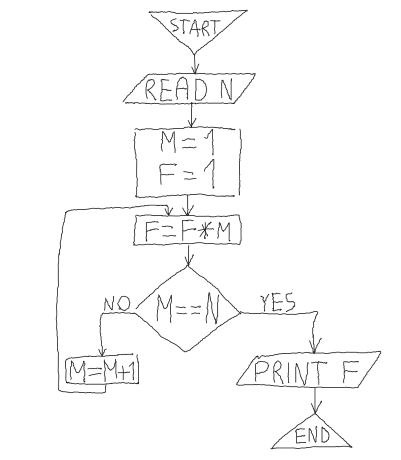
\includegraphics[scale=0.6]{Figure/diagram.PNG}
                    \caption{Esempio di sentenza visiva, da~\cite{localcontext_recognition}}
                    \label{fig:diagram}
                \end{figure}
                Ad esempio, come possiamo notare avvalendoci del disegno in figura~\ref{fig:diagram}, senza un contesto le forme grafiche sono soltanto simboli connessi fra loro da delle frecce. Invece, dando una definizione ai simboli può essere interpretato come un diagramma di flusso o \textit{Flowchart}\footnote{Il diagramma di flusso (o \textit{Flowchart}), in informatica, è una rappresentazione grafica delle operazioni da eseguire per l'esecuzione di un algoritmo.}.

            \subsection{Vantaggi}
                I vantaggi possono essere molteplici, innanzitutto un linguaggio visuale può essere molto più efficace e di facile comprensione rispetto al linguaggio verbale per via della sua semplicità e naturalità. Non ha lingue o convenzioni in quanto un disegno o un'immagine non dipende da lingue o standard.

    \section{Organizzazione della Tesi}
        Nel capitolo 2 illustrerò i lavori correlati al mio progetto di tesi.
        Nel capitolo 3 parlerò del Local Context e delle corrispondenti specifiche sintattiche e semantiche. 
        Nel capitolo 4 introdurrò il risultato del mio lavoro di tesi, TiveJS e le sue funzioni, e illustrerò  i dettagli dell'implementazione e le tecnologie usate. 
        Nel capitolo 5 illustrerò un esempio d'utilizzo. 
        Nel capitolo 6 presenterò possibili sviluppi futuri dell'applicazione e le conclusioni.

\chapter{Lavori Correlati}
    Il mio lavoro di tesi, essendo principalmente un porting ed una rivisitazione, si basa su strumenti precedentemente sviluppati. Gli strumenti in questione sono descritti nel dettaglio nei seguenti sotto-paragrafi.
    \newline
    La base teorica su cui si basa il mio lavoro è la definizione di un framework, chiamato \textbf{Local Context}, illustrato nel dettaglio nel capitolo 3.

    \section{Draw.io e mxGraph}

        \begin{figure}[htbp]
            \centering
            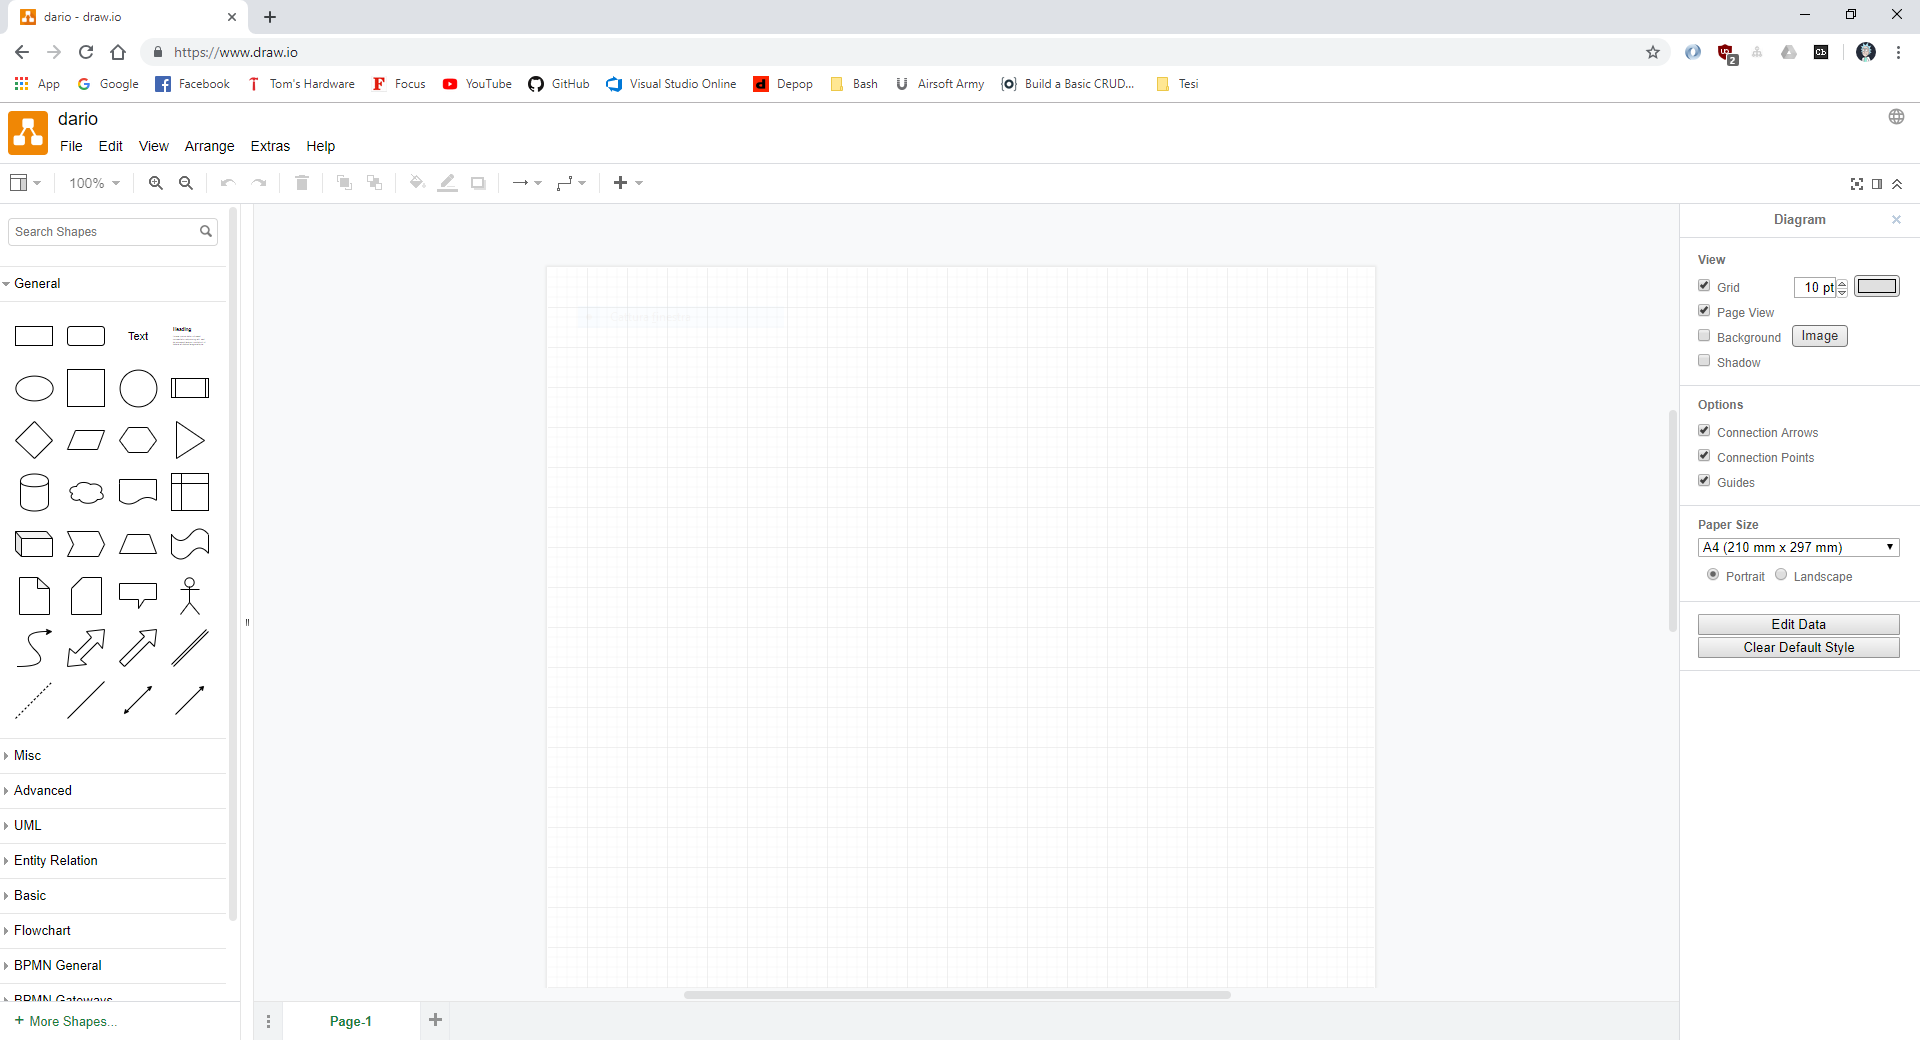
\includegraphics[scale=0.17]{Figure/drawio.png}
            \caption{Schermata di draw.io}
            \label{fig:drawio}
        \end{figure}

        TiveJS, è basato su draw.io, un'applicazione web open source che permette agli utenti di creare diagrammi e grafi direttamente dal proprio browser web, mostrata in figura \ref{fig:drawio}. Ha un'integrazione con Google Drive e Dropbox per il salvataggio dati che può avvenire anche con l'ausilio del \texttt{localStorage} del browser o attraverso il salvataggio di file sulla macchina. Draw.io è basato sulla libreria mxGraph. Il software è sviluppato dal 2005 dalla JGraph Ltd.

    \section{LoCoMoTiVE}
        
        All'attuale stato dell'arte vi è l'ecosistema LoCoMoTiVE, ovvero un'unione di due software, LoCoModeler e TiVE. Presentato in~\cite{extending_localcontext} e~\cite{localcontext}, questo tool permette l'analisi semantica basata sul contesto locale, illustrata nel dettaglio nel capitolo~\ref{ch:localcontext}. Nei prossimi due paragrafi andrò ad illustrare singolarmente i due componenti di cui è composto.

        \subsection{LoCoModeler}
        
            \begin{figure}[htbp]
                \centering
                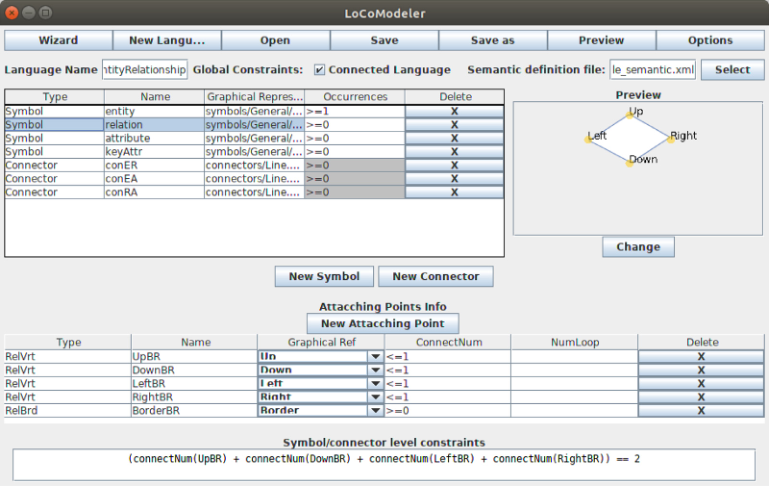
\includegraphics[scale=1.5]{Figure/locomodeler.png}
                \caption{Schermata di LoCoModeler \cite{localcontext}}
                \label{fig:locomodeler}
            \end{figure}

            Come descritto in \cite{extending_localcontext}, il modulo LoCoModeler consente ai designer la creazione e la modifica del linguaggio visivo in base al contesto locale, in maniera rapida e facile. Il suo output è la definizione in formato XML del linguaggio che verrà utilizzato durante il riconoscimento dei diagrammi. Una volta che il progettista ha completato la specifica del linguaggio, può compilarla in un ambiente web (il modulo TiVE) per consentire agli utenti di disegnare frasi e verificarne la correttezza. Durante la definizione del linguaggio, questa funzione consente al progettista di controllare la correttezza delle specifiche.
            \newline
            Una schermata principale dell'interfaccia grafica del tool è mostrata nella Figura \ref{fig:locomodeler}. Le sue componenti principali sono:
            \begin{itemize}
                \item Una casella di testo contenente il nome del linguaggio e una checkbox che sta ad indicare se il diagramma o grafo deve essere o non essere necessariamente connesso\footnote{Un grafo è detto connesso se, per ogni coppia di vertici $(u, v)\in{V}$, esiste un cammino che collega u a v.}.
                \item Una tabella riportante le informazioni principali dei simboli e dei connettori inclusi nel linguaggio. È possibile modificare o eliminare un elemento interagendo con la riga di quest'ultimo. L'utente può aggiungere nuovi simboli o connettori usando i bottoni sottostanti la tabella.
                \item Un pannello (sulla destra) mostra un'anteprima grafica del simbolo o connettore selezionato nella tabella. È possibile cambiare la rappresentazione grafica dell'elemento utilizzando il bottone \textit{Change}.
                \item Una tabella (al centro) mostra le informazioni relative al simbolo o connettore selezionato. Ogni riga mostra un punto d'attacco e i relativi vincoli. È possibile aggiungere nuove righe utilizzando i bottoni sovrastanti la tabella.
                \item Un'area di testo dove è possibile specificare i vincoli per il simbolo o il connettore attraverso espressioni simili al C\footnote{Linguaggio di programmazione.}.
            \end{itemize}
            La definizione di un nuovo linguaggio può avvenire grazie all'ausilio di un \textit{Wizard} diviso in tre fasi.

        \subsection{TiVE}

            \begin{figure}[htbp]
                \centering
                \includegraphics[scale=0.7]{Figure/tive.png}
                \caption{Schermata di TiVE}
                \label{fig:tive}
            \end{figure}

            Una volta definito il linguaggio, i diagrammi possono essere composti utilizzando i simboli e i connettori definiti nella sua specifica. Questo può essere fatto attraverso un editor grafico TiVE \cite{localcontext}, che è un'applicazione web che consente la composizione di diagrammi direttamente dal browser web.
            \newline
            Come mostrato nella Figura~\ref{fig:tive}, l'applicazione è costituita da tre sezioni principali:
            \begin{itemize}
                \item Nella toolbar a sinistra troviamo la palette dei simboli e connettori utilizzabili per la creazione dei diagrammi.
                \item Nella zona centrale troviamo l'area di lavoro dove è possibile comporre i diagrammi trascinando gli elementi contenuti nella toolbar di sinistra.
                \item A destra troviamo la Console dove verrà mostrata la traduzione semantica o la lista di errori nel caso in cui si verificassero.
            \end{itemize}

    \section{DrawSE}
        DrawSE è un'estensione di draw.io sviluppata in un precedente lavoro di tesi da Vincenzo Caputo. Questo software permette la creazione di diagrammi con simboli altamente personalizzati. Le principali caratteristiche di drawSE sono le due modalità di editing: una per la creazione di simboli (\textit{Shape Mode}) e una per la definizione dei punti d'attacco\footnote{Dove gli archi andranno ad attaccarsi sulla figura.} dei simboli (\textit{AP Mode}).
        Le due modalità sono attivabili attraverso il selettore mostrato in figura \ref{fig:mode_switch}
        \begin{figure}[htbp]
            \centering
            
\includegraphics[scale=0.7]{Figure/mode_switch.png}
            \caption{Switch per la selezione della modalità in drawSE}
            \label{fig:mode_switch}
        \end{figure}
        \newline
        La \textit{Shape Mode} permette la creazione di nuovi simboli e di personalizzarli in base al colore, lo spessore delle linee e così via. Un simbolo può essere formato anche dall'unione di più simboli semplici.
        Nella \textit{AP Mode}, drawSE fornisce una palette con sette strumenti utili alla definizione degli \textit{attaching point} del simbolo. Il punto d'attacco può essere composto da sette diverse forme geometriche:
        \begin{itemize}
            \item un punto
            \item una linea retta
            \item una linea curva
            \item un'area rettangolare
            \item un'area ellittica
            \item un contorno rettangolare
            \item un contorno ellittico
        \end{itemize}
        Altra funzionalità di drawSE è la creazione di set di simboli personalizzati o \textit{custom palette}, ovvero un insieme dei simboli creati grazie alle due modalità specificate prima. Lo strumento è spiegato nel dettaglio in \cite{drawSE}. TiveJS fa uso delle palette generate in drawSE.

\chapter{Linguaggi visuali}

    In questo capitolo entrerò nel dettaglio dei Linguaggi Visuali, andando ad illustrare quali sono le principali differenze tra un linguaggio visuale ed uno verbale, i componenti che lo compongono e in quali casi o contesti un linguaggi visivo è più efficace rispetto ad uno verbale.

    \section{Linguaggio verbale}
        Il linguaggio verbale è un gruppo di elementi, come suoni e parole, che messi insieme formano frasi e infine permettono la comunicazione fra individui. Da questo deriva la comunicazione verbale che è quindi costituita dalle parole usate quando parliamo o scriviamo.

    \section{Componenti}
        Ogni linguaggio è formato da un proprio insieme di componenti. Un linguaggio visuale si distingue principalmente dal linguaggio verbale per i componenti da cui è formato. Il linguaggio visivo si basa su simboli grafici o immagini, elementi che il cervello umano interpreta e trasforma in concetti, linguaggio verbale ed emozioni. Quindi se il linguaggio visuale è costituito da testo e parole per la formazioni di frasi, il linguaggio visivo è formato da simboli e disegni per formare sentenze visive.
        Una componente fondamentale di un linguaggio visuale è il contesto che viene dato ad ogni simbolo appartenente ad una frase visiva.
        \begin{figure}[htbp]
            \centering
            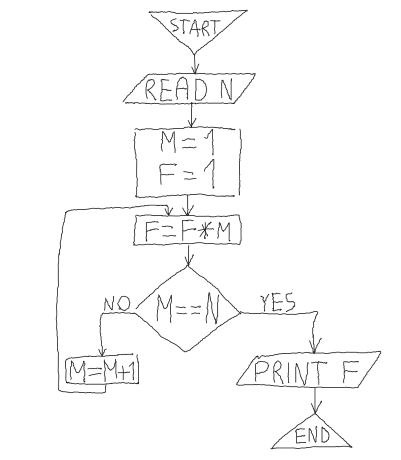
\includegraphics[scale=0.6]{Figure/diagram.PNG}
            \caption{Esempio di sentenza visiva, da~\cite{localcontext_recognition}}
            \label{fig:diagram}
        \end{figure}
        Ad esempio, come possiamo notare avvalendoci del disegno in figura~\ref{fig:diagram}, senza un contesto le forme grafiche sono soltanto simboli connessi fra loro da delle frecce. Invece, dando una definizione ai simboli può essere interpretato come un diagramma di flusso o \textit{Flowchart}\footnote{Il diagramma di flusso (o \textit{Flowchart}), in informatica, è una rappresentazione grafica delle operazioni da eseguire per l'esecuzione di un algoritmo.}.

    \section{Vantaggi}
        I vantaggi possono essere molteplici, innanzitutto un linguaggio visuale può essere molto più efficace e di facile comprensione rispetto al linguaggio verbale per via della sua semplicità e naturalità. Non ha lingue o convenzioni in quanto un disegno o un'immagine non dipende da lingue o standard.

\chapter{Local Context}\label{ch:localcontext}
    Il riconoscimento dei diagrammi viene effettuato in base al \textit{Local Context}, presentato nei paper~\cite{localcontext_recognition},~\cite{extending_localcontext} e~\cite{localcontext}.
    \newline
    Nel paper \textit{Local context-based recognition of sketched diagrams} \cite{localcontext_recognition}, il Local Context viene presentato come una nuova metodologia mirata alla creazione e all'implementazione di un framework\footnote{\textit{"Un framework, in generale, include software di supporto, librerie, un linguaggio per gli script e altri software che possono aiutare a mettere insieme le varie componenti di un progetto." \cite{framework}}} per il riconoscimento e l'interpretazione dei diagrammi. Nello specifico, i diagrammi possono contenere differenti elementi grafici quali simboli, connettori e testo. Una volta che i simboli sono stati identificati, il riconoscimento procede identificando il contesto locale di ogni simbolo.
    Il Local Context ha due diverse specifiche: sintattiche e semantiche.
    \section{Sintassi}
        Sempre in~\cite{localcontext_recognition}, viene definita la specifica sintattica di un linguaggio visuale.
        In particolare, usando il contesto locale, la specificazione della sintassi di un linguaggio visivo consiste di svariati elementi:
        \begin{itemize}
            \item Definizione dei simboli (token) che compongono il linguaggio visuale:
            \begin{itemize}
                \item Definizione dell'apparenza "fisica" dei simboli (ad esempio forma, colore, ecc.);
                \item Definizione degli attributi del simbolo della loro forma e del loro aspetto (ad esempio punti/area d'attacco, ecc);
                \item Definizione dei vincoli locali al simbolo riguardanti gli attributi (ad esempio il numero di connessioni permesse ad un punto d'attacco, ecc.).
            \end{itemize}
            \item Definizione delle relazioni/connettori e i loro vincoli locali;
            \item Dichiarazione di vincoli al livello del diagramma (ad esempio numero di occorrenze ammissibili di un simbolo, se i simboli e i connettori devono formare un grafo connesso);
            \item Una grammatica per definire ulteriori vincoli di sintassi del linguaggio (quando necessario).
        \end{itemize}

        \begin{table}[htbp]
            \centering
            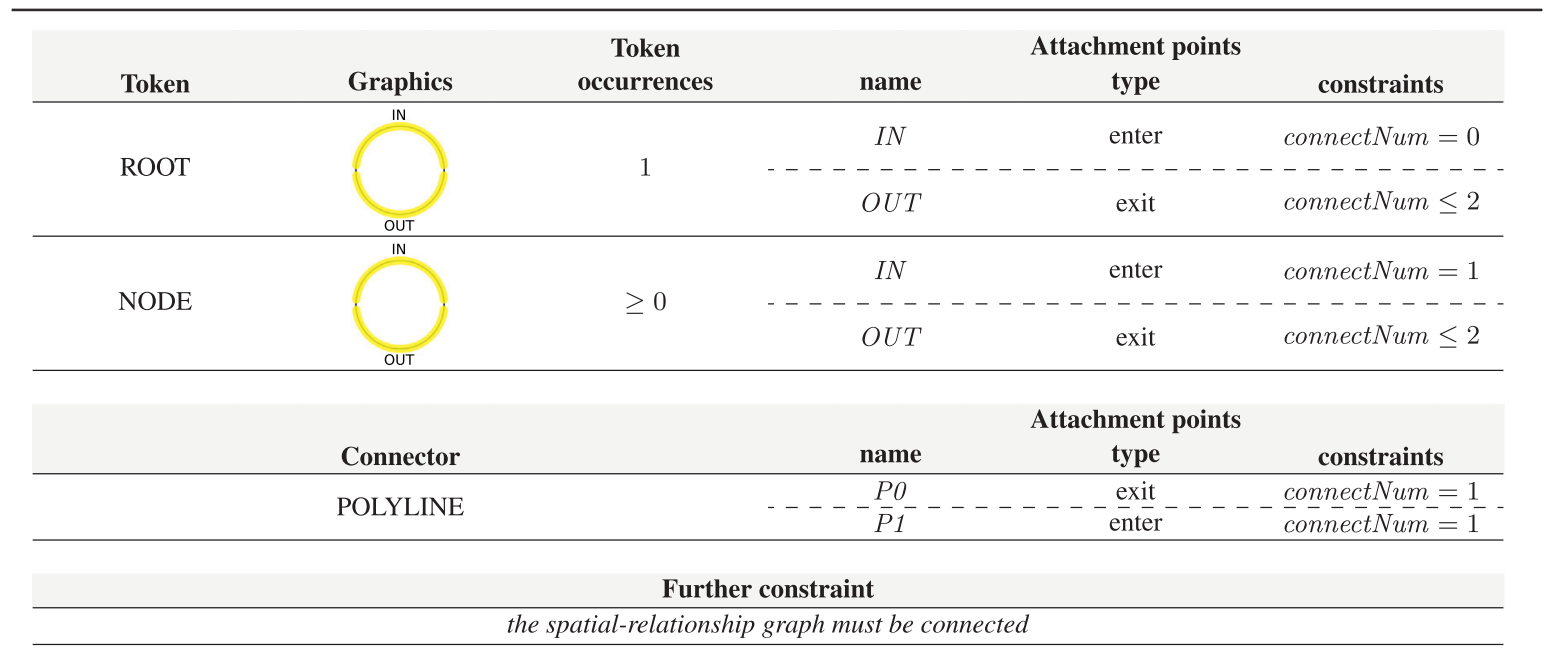
\includegraphics[scale=0.35]{Figure/elem_specification.PNG}
            \caption{Specifica di un linguaggio, nel particolare di un Albero \cite{localcontext_recognition}}
            \label{tab:elem_specification}
        \end{table}
        \noindent
        Facendo riferimento alla tabella~\ref{tab:elem_specification}, ovvero la specifica di un linguaggio che identifica un Albero, possiamo notare che ogni riga identifica un simbolo (o token) e che ogni riga è composta da sei colonne, le prime tre sono indirizzate al livello del simbolo e le restanti tre colonne indicano i vincoli per gli attachment points:
        \begin{itemize}
            \item \textbf{Token}: indica il nome dell'elemento;
            \item \textbf{Graphics}: rappresentazione grafica dell'elemento e rappresentazione dei punti d'attacco evidenziati in giallo;
            \item \textbf{Token occurences}: numero di occorrenze ammissibile per quel simbolo;
            \item \textbf{name}: può essere composta da più righe ed indica i nomi dei punti d'attacco;
            \item \textbf{type}: la tipologia di AP\footnote{Punti d'attacco.}, un tipo di punto di attacco può avere più nomi;
            \item \textbf{constraints}: i vincoli al livello dei punti d'attacco, \textit{connectNum} indica il numero di archi incidenti a quel determinato AP.
        \end{itemize}
        I vincoli al livello della sentenza sono riportati nell'ultima riga. Una parte della formalizzazione della tabella \ref{tab:elem_specification} in formato XML è mostrata nello snippet di codice \ref{lst:xml_elem_specification}, l'intera specifica è consultabile nell'appendice \ref{appendix:xml_definition}.

        \lstinputlisting[language=JavaScript,caption={\textbf{Frammento della definizione in formato XML di un linguaggio, nel particolare la specifica per il simbolo \textit{root} (o radice).}},label={lst:xml_elem_specification},language=Xml, firstline=2, lastline=7]{SourceCode/tree_specific.xml}

        \noindent
        Nel paper~\cite{extending_localcontext}, viene esteso il concetto esposto in~\cite{localcontext_recognition} aggiungendo nuove caratteristiche alla specifica del contesto locale per permettere la specifica di linguaggi visuali più complessi quali diagrammi entità-relazione, use case diagrams e class diagram. In più viene presentato un tool (LoCoMoTiVE, specificato nel paragrafo 2.2) che implementa il framework \textit{Local Context}.
        \newline
        Le principali caratteristiche aggiunte sono tre:
        \begin{itemize}
            \item La definizione di vincoli al livello del simbolo può coinvolgere più di un area di attacco di un simbolo/connettore al contrario di vincolare aree d'attacco individuali;
            \item La definizione di un vincolo per limitare auto-cicli di un connettore;
            \item Assegnazione di più tipi alle aree di attacco.
        \end{itemize}

    \section{Semantica}
        \label{sec:semantica}
        In \cite{localcontext} viene esteso il framework definendo una nuova tecnica per una traduzione semantica del linguaggio visuale basata sul contesto locale. Questa tecnica usa delle espressioni simili a queli di XPath, chiamate SGPath, illustrate nel dettaglio nel capitolo 5.
        \newline
        Per consentire la traduzione semantica di un linguaggio visuale è stata descritta una definizione semantica basata sul contesto locale o \textit{LCSD}\footnote{Local Context-based Semantic Definition} e il suo algoritmo per valutarla. L'LCSD consiste di una sequenza di regole semantiche, una per ogni elemento del linguaggio. Ogni regola calcola una proprietà attraverso delle procedure che fanno uso degli SGPath o esegue un'azione. Ogni proprietà può avere una post-condizione.
        \newline
        Attraverso le post-condizioni, una LCSD può dare una definizione migliore della struttura sintattica; attraverso le azioni restituisce una traduzione delle sentenze. Un'azione può dipendere dalle proprietà e dagli attributi dell'elemento.
        \begin{table}[htbp]
            \centering
            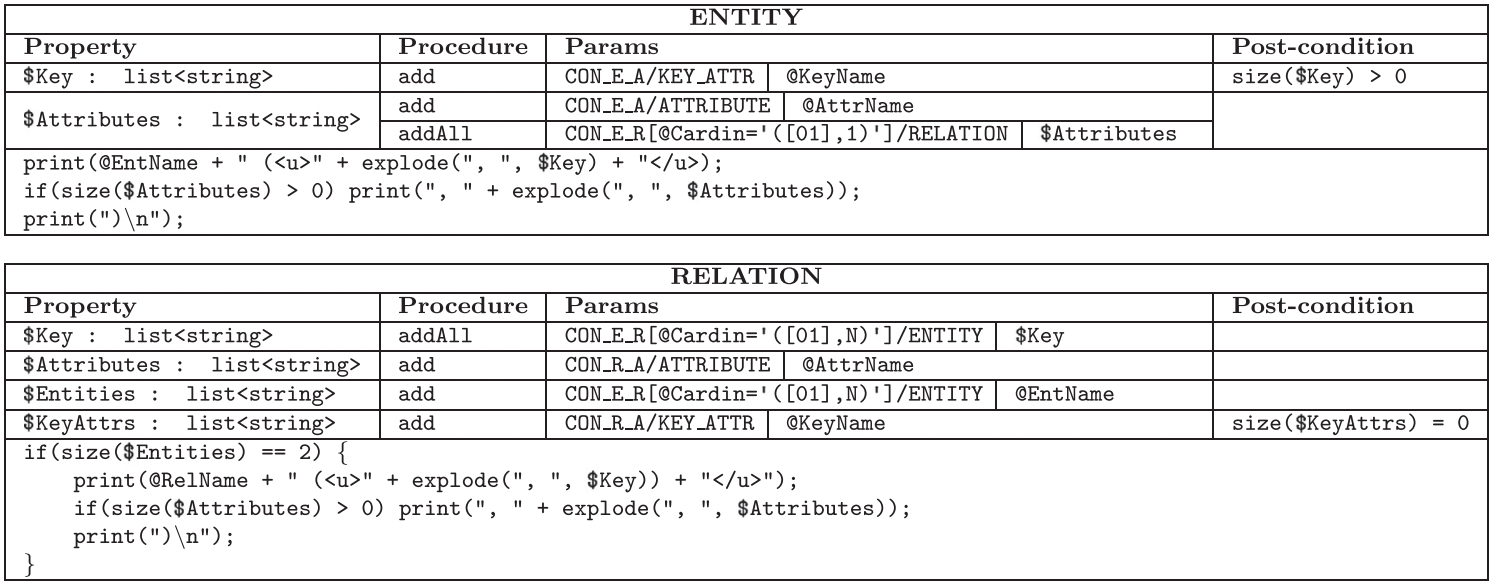
\includegraphics[scale=0.37]{Figure/semantic_specification.PNG}
            \caption{Specifica LCSD di un diagramma ER, costruita sulla specifica sintattica \cite{localcontext}}
            \label{tab:semantic_specification}
        \end{table}
        \newline
        La tabella \ref{tab:semantic_specification} mostra una specifica semantica di un diagramma ER\footnote{Entità Relazione.}. Ogni tabella fornisce le regole semantiche di un elemento, in questo caso per i simboli ENTITY e RELATION, rispettivamente. Ogni riga della specifica è composta dai seguenti elementi:
        \begin{itemize}
            \item \textbf{Property}: indica il nome della proprietà (preceduta dal carattere \$) e il tipo di variabile contenuta.
            \item \textbf{Procedure}: indica il nome della procedura da utilizzare per assegnare/modificare il valore di una proprietà, ogni proprietà può avere più procedure.
            \item \textbf{Params}: i parametri da utilizzare nella procedura. Il primo parametro è un SGPath, il secondo parametro è il nome della proprietà dove leggere le informazioni del/i simbolo/i raggiungibile/i con quel percorso.
            \item \textbf{Post-condition}: la post-condizione che deve essere rispettata al termine dell'esecuzione della procedura. 
        \end{itemize}
        L'ultima colonna indica l'azione da eseguire. A differenza dell'attuale implementazione, TiVeJS può eseguire anche azioni parziali, ovvero posizionata tra le proprietà e non dopo le proprietà.
        \newline
        \begin{figure}[htbp]
            \centering
            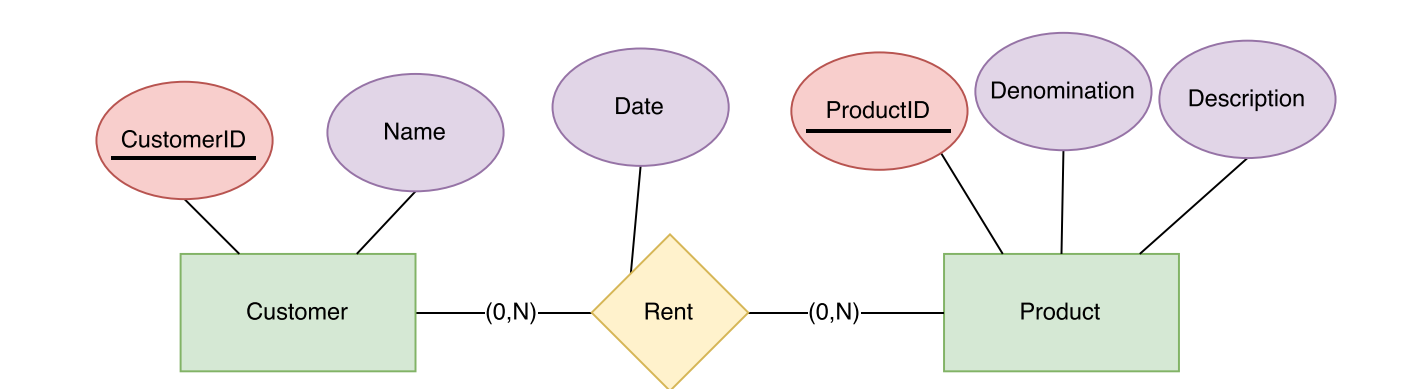
\includegraphics[scale=0.4]{Figure/er_diagram.PNG}
            \caption{Diagramma ER, \cite{localcontext}}
            \label{fig:er_diagram}
        \end{figure}
        In questo caso, applicando le regole semantiche definite nella tabella \ref{tab:semantic_specification} al diagramma \ref{fig:er_diagram} ottengo la seguente traduzione semantica:
        \begin{quotation}
            \noindent
            Customer (\underline{CustomerID}, Name) \newline
            Product (\underline{ProductID}, Denomination, Description) \newline
            Rent (\underline{CustomerID, ProductID}, Date)
        \end{quotation}
        Tutti i dettagli implementativi saranno illustrati nel prossimo capitolo.

\chapter{TiveJS}
    Come introdotto, in questo lavoro presento TiveJS, che è un porting ed un'evoluzione di TiVE e come esso è in grado di: permettere la progettazione di sentenze visive grazie all'ausilio di palette di simboli personalizzate, il riconoscimento di linguaggio diagrammatici e la traduzione di quest'ultimi.
    \newline
    Per l'implementazione di TiveJS mi sono basato sulle specifiche illustrate nel paper \textit{Using the local context for the definition and implementation of visual languages}~\cite{localcontext} in cui viene illustrato un metodo per la traduzione di diagrammi o in generale di sentenze visuali in sentenze semantiche.

    \section{Implementazione}
        L'applicazione si divide principalmente tre fasi, mostrate schematicamente nella figura~\ref{fig:funzionamento}: la progettazione del diagramma, il riconoscimento di quest'ultimo e l'applicazioni delle definizioni sintattiche e semantiche. Durante tutte le procedure, la navigazione all'interno del grafo viene effettuata attraverso delle espressioni chiamate SGPath.
        \newline
        \begin{figure}[htbp]
            \centering
            \smartdiagramset{border color=none,
                back arrow disabled=true,
                text width=3.5cm,
                module minimum width=3.5cm,
                module x sep=5
            }
            \smartdiagram[flow diagram:horizontal]{Progettazione, Riconoscimento, Applicazione Definizioni}
            \caption{Diagramma del funzionamento di TiveJS}
            \label{fig:funzionamento}
        \end{figure}

        Come vedremo, ogni fase può suddividersi in più sotto-fasi illustrate nel dettaglio nelle prossime sezioni.

        \subsection{SGPath}
            In questa sezione riassumo il lavoro svolto in \cite{localcontext} in cui viene descritta una specifica simile a XPath\footnote{\textit{"In informatica XPath è un linguaggio, parte della famiglia XML, che permette di individuare i nodi all'interno di un documento XML. Le espressioni XPath, a differenza delle espressioni XML, non servono a identificare la struttura di un documento, bensì a localizzarne con precisione i nodi."} \cite{xpath}} per la navigazione all'interno del grafo chiamata SGPath. Mentre XPath definisce delle espressioni per la navigazione all'interno dei file XML, SGPath definisce delle espressioni per navigare in una struttura a grafo.
            \newline
            Un SGPath consiste di passaggi (o \textit{step}). Ogni passo è valutato su un insieme di nodi del grafo. Il risultato di ogni passo è un insieme di nodi del grafo. SGPath può far uso delle proprietà dei simboli quali nome, id, ecc.
            \newline
            La sintatssi di un SGPath è strutturata in questo modo:
            \begin{quotation}
                \texttt{sgpath\_step\_1/sgpath\_step\_2/ … /sgpath\_step\_n}
            \end{quotation}
            ogni sgpath\_step è formato in questo modo:
            \begin{quotation}
                \texttt{axis(edge-filter)::node-test[predicate]}
            \end{quotation}
            dove:
            \begin{itemize}
                \item \textbf{axis(edge-filter)::} è opzionale e indica come continuare la navigazione partendo dal nodo corrente. A differenza di XPath, concede di spostari solo tra nodi adiacenti.
                \item \textbf{node-test} indica il nodo da raggiungere. Può essere il nome di un elemento o * per indicare qualsiasi nodo.
                \item \textbf{\lbrack predicate\rbrack} è opzionale e permette di selezionare i nodi con attributi specifici.
            \end{itemize}
            Ecco alcuni esempi di SGPath:
            \begin{itemize}
                \item \texttt{CON\_E\_A/KEY\_ATTR}
                \item \texttt{CON\_E\_R[@Cardin='([01],N)']/ENTITY}
                \item \texttt{(\#attName = 'Up')::ARROW/PRED}
                \item \texttt{(\#attName = 'Up')::ARROW/*}
            \end{itemize}
            In TiveJS l'algoritmo che si occupa della risoluzione degli SGPath è visibile all'interno dello snippet \ref{lst:resolvePath}. La funzione \texttt{resolvePath} divide la stringa al carattere '\texttt{/}' così da ottenere ogni step del percorso. A questo punto ogni step viene scorporato di tutti i suoi campi dalla funzione \texttt{scorporatePath} che restituisce un oggetto con all'interno tutte le informazioni sul singolo step.
            \begin{lstlisting}[language=JavaScript,caption=\textbf{Funzione che si occupa della risoluzione delle path},label={lst:resolvePath}]
                /**
                * Resolve path
                */
                CheckUtil.prototype.resolvePath = function (node, path) {
                    console.log('RESOLVING A PATH FOR: ' + node.id);
                    console.info('node, path', node, path);
                    let nodes = [];
                    nodes = nodes.concat(node);
                    let splittedPath = path.split('/');
                    for (let elem in splittedPath) {
                        let pathStep = splittedPath[elem];
                        nodes = this.resolvePathStep(nodes, pathStep);
                    }
                    console.info('returned nodes', nodes);
                    return nodes;
                }
            \end{lstlisting}
        \newpage
        \subsection{Progettazione di sentenze visive}
            La progettazione delle sentenze visive avviene attraverso una GUI\footnote{Interfaccia Grafica.} molto semplice ed intuitiva, simile a quella nella figura~\ref{fig:drawio}.

            \begin{figure}[htbp]
                \centering
                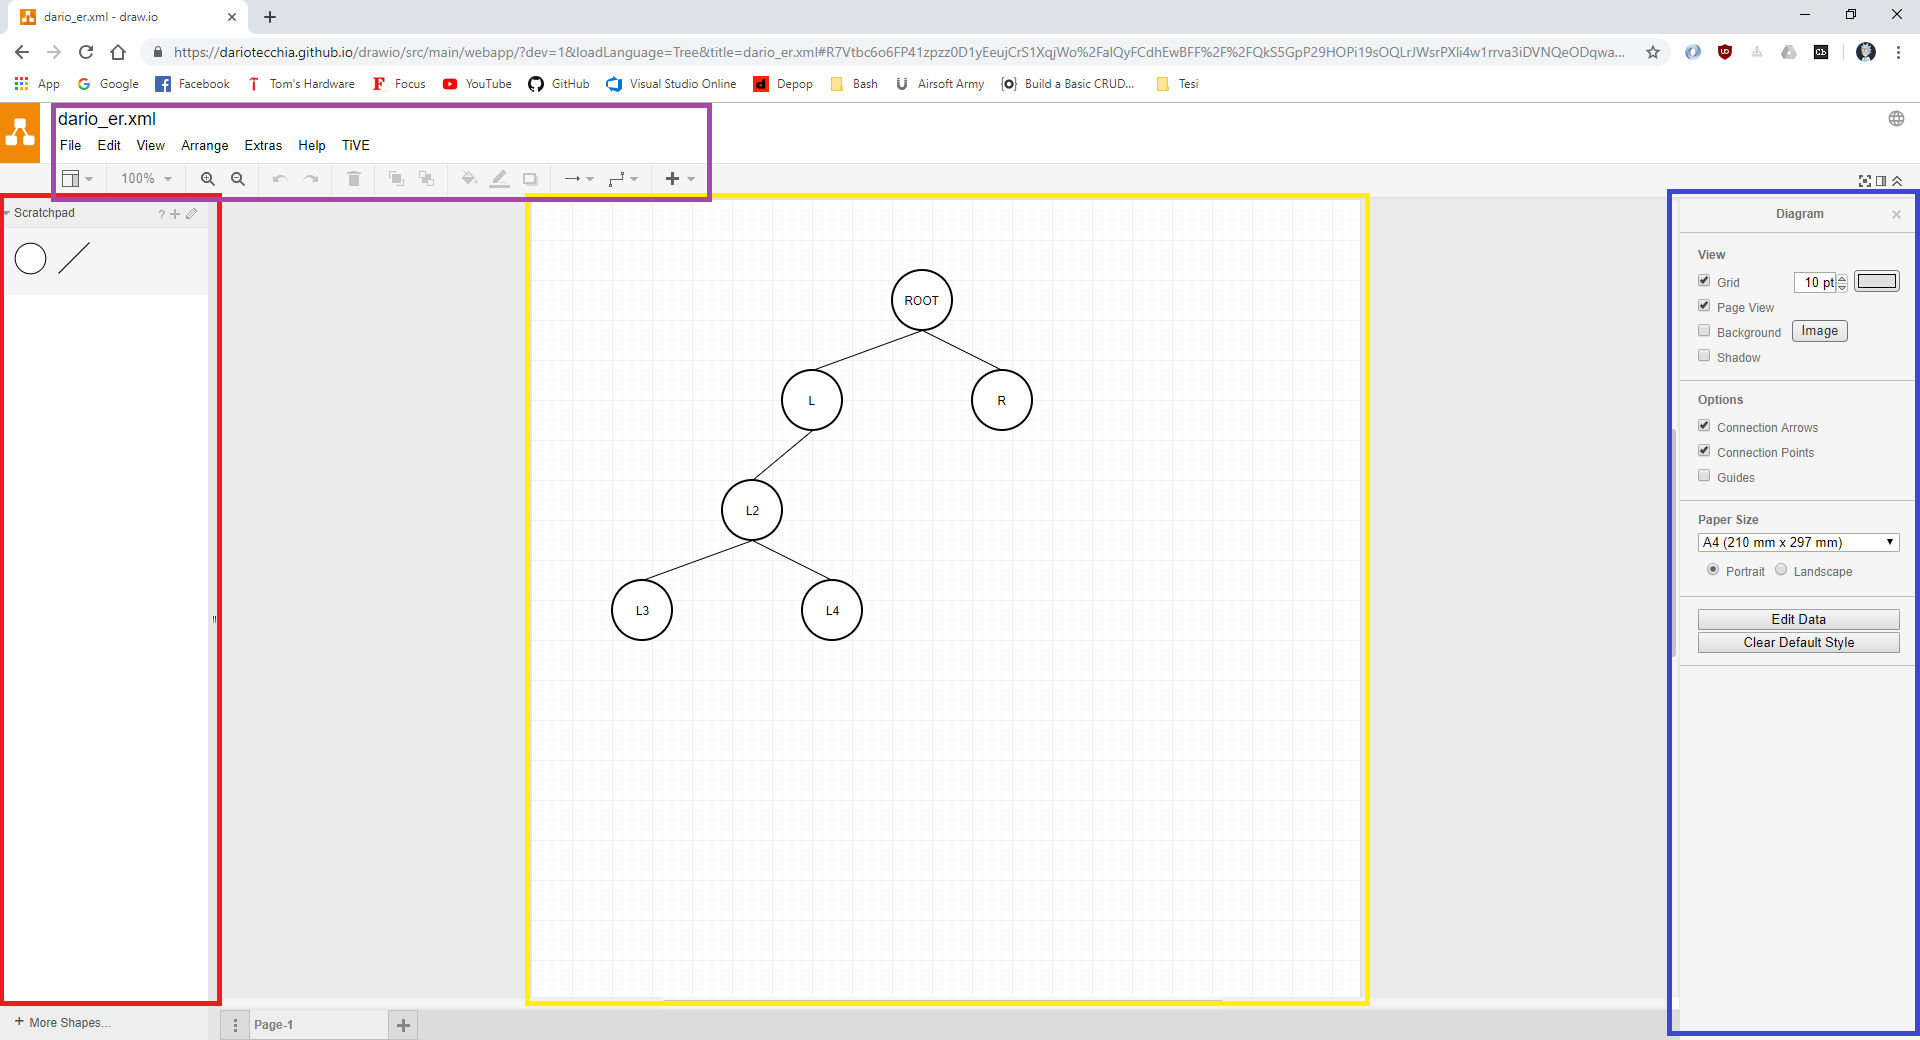
\includegraphics[scale=0.25]{Figure/tivejs_gui2.png}
                \caption{Schermata principale di TiveJS}
                \label{fig:tivejsgui}
            \end{figure}

            E' composta di quattro sezioni principali (figura~\ref{fig:tivejsgui}):
            \begin{itemize}
                \item Barra laterale sinistra (evidenziata \textcolor{red}{rosso})
                \item Barra laterale destra (evidenziata \textcolor{blue}{blu})
                \item Area di lavoro (evidenziata \textcolor{yellow}{giallo})
                \item Barra dei menu (evidenziata \textcolor{purple}{viola})
            \end{itemize}
            All'interno della barra laterale sinistra c'è la palette dei simboli importata precedentemente creata con l'ausilio di \textit{drawSE}. Per importare una nuova libreria (o palette) bisogna andare nel menu \textit{File -> Open Library From} e selezionare il metodo di importazione.
            \newline
            La barra laterale destra serve a personalizzare ulteriormente il diagramma o il singolo simbolo. Mette a disposizione vari menù ed opzioni quali la dimensione della pagina su cui disegnamo il diagramma, il colore di un simbolo, le proprietà del testo contenuto all'interno di un simbolo, ecc. 
            \newline
            L'area di lavoro è dove viene composto il diagramma trascinando i simboli dalla barra laterale. All'interno di quest'area possiamo selezionare, modificare e spostare il diagramma e i relativi simboli a nostro piacimento.
            \newline
            La barra dei menu è composta da tanti sotto menu ognuno dei quali ha una funzione specifica. Oltre ai menu di draw.io, ho aggiunto un nuovo menu "TiVE" (figura \ref{fig:tivemenu}) per il caricamento delle definizioni e per la verifica del grafo. Nello specifico, "\textit{Load Rules...}" serve per il caricamento delle definizioni sintattiche; "\textit{Load Semantic Rules...}" serve per il caricamento delle definizioni semantiche e "\textit{Apply Rules}" serve ad eseguire l'applicazione di quest'ultime e ad eseguire la traduzione semantica del diagramma.
            
            \begin{figure}[htbp]
                \centering
                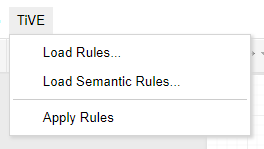
\includegraphics[]{Figure/tive_menu.PNG}
                \caption{Menu dei comandi per TiVE}
                \label{fig:tivemenu}
            \end{figure}

        \subsection{Riconoscimento grafo}
            All'interno del diagramma, più simboli con scopi diversi possono condividere lo stesso elemento grafico creando delle ambiguità. Una delle prime fasi del processo di traduzione è il riconoscimento degli elementi e quindi la risoluzione di queste ambiguità. Come possiamo notare nella tabella~\ref{tab:final_syntax_definition}, in particolare nella seconda sotto-tabella, i connettori pur avendo uno scopo diverso condividono lo stesso elemento grafico, una linea.
            \newline
            Ancora, nella tabella \ref{tab:final_syntax_definition_tree} a condividere lo stesso elemento grafico è un simbolo: ROOT e NODE sono entrambi rappresentati da un cerchio.

            \begin{table}[htbp]
                \centering
                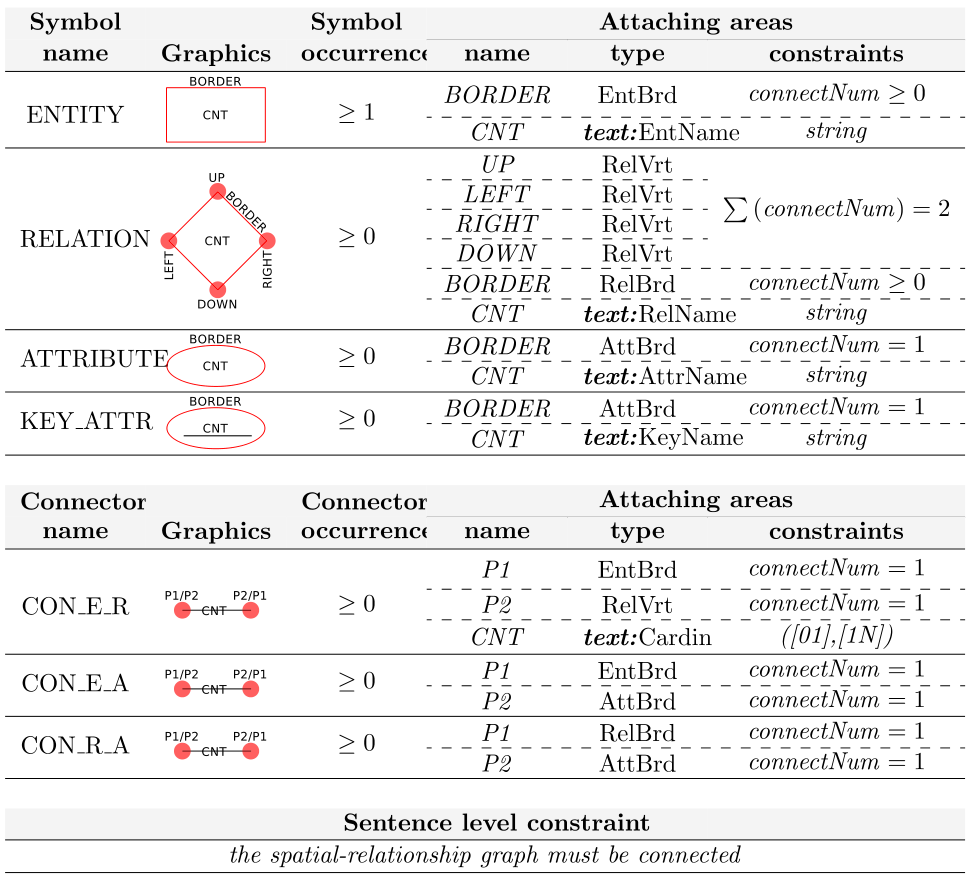
\includegraphics[scale=0.4]{Figure/final_syntax_definition.PNG}
                \caption{Specifica di un diagramma ER \cite{localcontext}}
                \label{tab:final_syntax_definition}
            \end{table}

            \begin{table}[htbp]
                \centering
                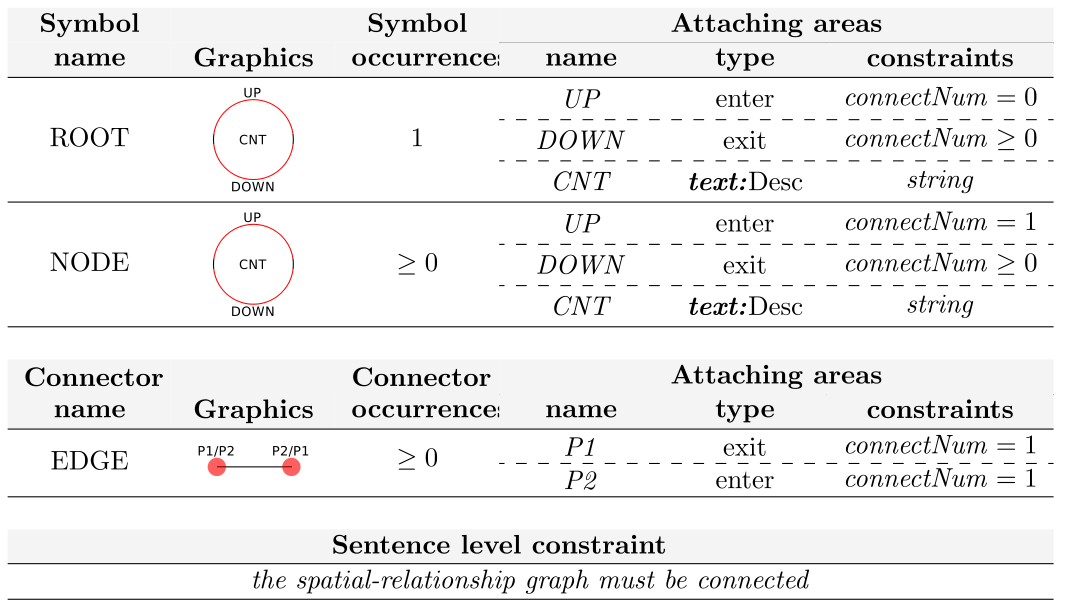
\includegraphics[scale=0.4]{Figure/final_syntax_definition_tree.PNG}
                \caption{Specifica di un Albero \cite{localcontext}}
                \label{tab:final_syntax_definition_tree}
            \end{table}

            A caratterizzare un elemento sono le proprietà della definizione sintattica correlata e la disambiguazione viene effettuata tenendo in considerazione questi elementi.
            \newline
            L'algoritmo risolutivo innanzitutto rileva se si sta analizzando un vertice o un connettore e nel caso in cui venissero rivelate delle ambiguità procede come segue: Se l'elemento analizzato è un connettore prende in considerazione il campo \textit{Type} delle due aree d'attacco. All'interno di questa proprietà vengono indicati i tipi di area d'attacco in cui il connettore è collegato alle due estremità. Ad esempio, il connettore \textit{CON\_E\_A} (Connettore Entità-Attributo) alle due estremità si connetterà ad una \textit{EntBrd} e ad una \textit{AttBrd} in posizioni arbitrali; Nel caso un cui l'elemento analizzato è un vertice allora il controllo viene effettuato sui vincoli definiti per ogni simbolo. Il vertice sarà associato al simbolo per cui verranno rispettati tutti i suoi vincoli. Ad esempio, il simbolo ROOT dovrà avere un numero di connessioni (\textit{connectNum}) uguali a zero sull'attaching area UP di tipo enter e un numero maggiore o uguale a zero di connessioni sull'attaching area DOWN di tipo exit.
            \newline

        \subsection{Applicazione definizioni}
            Eseguito il riconoscimento di ogni simbolo appartenente al grafo, l'algoritmo procede con l'applicazione delle definizioni. Come ho già accennato, la specifica delle definizioni si divide in due parti: sintattica e semantica.

            \subsubsection{Definizioni Sintattiche}
                Ogni linguaggio ha delle regole sintattiche da rispettare. Un esempio di definizione sintattica è raffigurata nella tabella \ref{tab:final_syntax_definition}. Nella colonna \textit{Symbol occurences} vi è un vincolo al livello del simbolo, indica quante occorrenze del simbolo devono essere presenti all'interno del diagramma. Nell'ultima colonna, \textit{constraints}, vi troviamo i vincoli al livello degli Attaching Point e il formato che deve avere il campo di testo dell'elemento se specificato. Nell'ultima riga, \textit{Sentence level constraint}, troviamo i vincoli che il diagramma deve rispettare.
                \newline
                Come ho già accennato, in TiVE le definizioni erano scritte in formato XML (vedi Appendice \ref{appendix:xml_definition}). Successivamente le ho implementate in formato JSON\footnote{JavaScript Object Notation}, seguendo uno schema (\ref{appendix:syntaxSchema}) da me definito, per poter essere interpretate in maniera nativa dal linguaggio di programmazione da me usato. All'interno dello snippet di codice \ref{lst:newDefinition} vi è una parte della definizione nel nuovo formato. 
                \begin{spacing}{0.5}
                    \lstinputlisting[language=JavaScript, caption={\textbf{Frammento della definizione sintattica in formato JSON di un linguaggio, nel particolare la specifica per il simbolo \textit{ROOT} (o Radice).}},label={lst:newDefinition}, firstline=4, lastline=29]{SourceCode/newDefinition.json}
                \end{spacing}
                \begin{itemize}
                    \item \textbf{ap} è un array contenente i vincoli per i punti d'attacco;
                    \item \textbf{text} contiene le informazioni riguardanti le aree di testo;
                    \item \textbf{\_name} è il nome del simbolo;
                    \item \textbf{\_ref} indica a quale figura grafica si fa riferimento;
                    \item \textbf{occurences} è il vincolo sulle occorrenze del simbolo.
                \end{itemize}
                L'intera definizione d'esempio è consultabile all'Appendice \ref{appendix:jsonDefinition}.

            \subsubsection{Definizioni Semantiche}
                Le definizioni semantiche sono necessarie alla traduzione del diagramma. Un esempio di definizione semantica (o definizione LCSD) è raffigurata nella tabella \ref{tab:semantic_specification}. Come già detto nella sezione \ref{sec:semantica}, la specifica semantica è composta da quattro elementi fondamentali: 
                \begin{itemize}
                    \item \textbf{Property} indica il nome della proprietà semantica da attribuire all'elemento della specifica;
                    \item \textbf{Procedure} è il nome della procedura da utilizzare per assegnare o modificare la proprietà;
                    \item \textbf{Params} sono i parametri da passare alla procedura;
                    \item \textbf{Post-condition} è la condizione che deve essere rispettata al termine dell'esecuzione della procedura.
                \end{itemize}
                Anche in questo caso ho trascritto le definizioni sintattiche dal formato XML al formato JSON utilizzando uno schema da me definito (\ref{appendix:semanticSchema}). All'interno dello snippet di codice \ref{lst:newSemanticDefinition} vi è una parte della definizione nel nuovo formato. 
                \begin{itemize}
                    \item \textbf{property} contiene tutte le proprietà da computare. Ogni proprietà è composta da:
                    \begin{itemize}
                        \item \textbf{\_name} è il nome della proprietà;
                        \item \textbf{\_type} è il formato della proprietà;
                        \item \textbf{procedure} contiene le procedure da eseguire. Ogni procedura è composta da:
                        \begin{itemize}
                            \item \textbf{\_postCondition} è la condizione da rispettare al termine della procedura;
                            \item \textbf{name} è il nome della procedura;
                            \item \textbf{\_path} insieme a \textbf{\_param} sono i parametri da passare alla procedura.
                        \end{itemize}
                    \end{itemize}
                    \item \textbf{visit} verrà utilizzato dall'algoritmo di ordinamento del grafo.
                \end{itemize}
                L'intera definizione è consultabile all'Appendice \ref{appendix:ERjsonSemanticDefinition}.
                \newpage
                \begin{spacing}{0.5}
                    \lstinputlisting[language=JavaScript, caption={\textbf{Frammento della definizione semantica in formato JSON di un linguaggio, nel particolare la specifica per il simbolo STAT}},label={lst:newSemanticDefinition}, firstline=200, lastline=241]{SourceCode/EXAMPLES/flowchartp/newSemanticDefinition.json}
                \end{spacing}

        \subsection{Applicazione Regole Semantiche}
            Se l'applicazione delle definizioni è andata a buon fine, l'algoritmo procede con il calcolo delle regole semantiche. La procedura si suddivide in due fasi: ordinamento del grafo e calcolo delle definizioni semantiche.

            \subsubsection{Ordinamento del grafo}
                In precedenza ho parlato del campo \textit{visit} presente all'interno della definizione semantica di un linguaggio. Questo campo serve a costruire una \textit{Visit Table} necessaria a definire l'ordine in cui gli elementi del diagramma verranno visitati dall'algoritmo.

                \begin{table}[htbp]
                    \centering
                    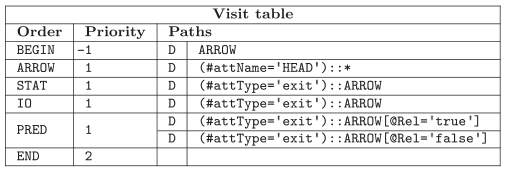
\includegraphics[scale=0.6]{Figure/visitTable.PNG}
                    \caption{Visit Table per il linguaggio Flowchart}
                    \label{tab:visitTable}
                \end{table}

                Ogni simbolo ha una priorità, come mostrato nella tabella \ref{tab:visitTable}. Questa tabella specifica la priorità per ogni elemento del linguaggio flowchart, in particolare -1 per il simbolo BEGIN, 2 per il simbolo END e 1 per tutti gli altri simboli. In questo modo il simbolo BEGIN verrà posizionato all'inizio, END alla fine e gli altri simboli in una posizione arbitraria. 
                \newline
                La colonna \textit{Paths} della tabella indica il prossimo nodo da esplorare, se presente. Questa è composta da due sezioni, una è un flag che indica se l'esplorazione viene effettuata in ampiezza (B) o un profondità (D) e l'altra è il percorso da seguire.
                \newline
                Altro modo di definire un ordine è con la \textit{Path Table}, mostrata nella tabella \ref{tab:pathTable}. 

                \begin{table}[htbp]
                    \centering
                    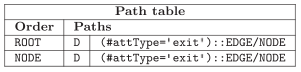
\includegraphics[scale=0.85]{Figure/pathTable.PNG}
                    \caption{Path Table per il linguaggio Tree}
                    \label{tab:pathTable}
                \end{table}

                La tabella di visita viene applicata al diagramma dalla funzione \texttt{ApplyVisitTable} (snippet \ref{lst:applyVisitTable}) che fa uso di un'altra funzione fondamentale, \texttt{FollowPath} (snippet \ref{lst:followPath}).
                \newpage
                \begin{lstlisting}[language=JavaScript, basicstyle=\tiny, caption={La funzione applyVisitTable}, label={lst:applyVisitTable}]
                    // Apply the visit table to the graph
                    CheckUtil.prototype.applyVisitTable = function (graph, visitTable) {
                        let N = Object.values(graph).sort((a, b) => {
                            return visitTable[a.name].order - visitTable[b.name].order;
                        });
                        let L = [];
                        while (N.length != 0) {
                            let rem = N.shift();
                            L.push(rem);
                            let nodes = [];
                            nodes = this.followPath(rem, graph, N, visitTable, nodes);
                            L = L.concat(nodes);

                            N = N.filter((i) => {
                                return nodes.indexOf(i) < 0;
                            });
                        }

                        L = this.stableSort(L, (a, b) => {
                            if (visitTable[a.name].priority > visitTable[b.name].priority) {
                                return 1;
                            }
                            if (visitTable[a.name].priority < visitTable[b.name].priority) {
                                return -1;
                            }
                        });
                        return L;
                    }
                \end{lstlisting}

                \begin{lstlisting}[language=JavaScript, basicstyle=\tiny, caption={La funzione followPath}, label={lst:followPath}]
                    // Follow the path from a node
                    CheckUtil.prototype.followPath = function (node, G, N, PTPATHS, nodes) {
                        let nname = node.name;
                        let npaths = PTPATHS[nname].paths;
                        for (let elem in npaths) {
                            let npath = npaths[elem];
                            let nds = this.resolvePath(node, npath._value);
                            nds = nds.filter((i) => {
                                return nodes.indexOf(i) < 0;
                            });
                            nds = nds.filter((i) => {
                                return N.indexOf(i) > -1;
                            });
                            if (npath._flag == 'B') {
                                nodes = nodes.concat(nds);
                            }
                            for (let elem in nds) {
                                let n = nds[elem];
                                if (npath._flag == 'D') {
                                    if (nodes.indexOf(n) < 0) {
                                        nodes.push(n);
                                    }
                                }
                                nodes = this.followPath(n, G, N, PTPATHS, nodes);
                            }
                        }
                        return nodes;
                    }
                \end{lstlisting}
                \newpage
                Ordinato il grafo, l'algoritmo procede con l'applicazione delle definizioni semantiche.
                
            \subsubsection{Calcolo definizioni semantiche}
                Altro ruolo importante è quello della funzione \texttt{ApplySemanticRules} (snippet \ref{lst:applySemanticRules}).

                \begin{lstlisting}[language=JavaScript, basicstyle=\tiny, caption={La funzione che computa tutte le proprietà semantiche}, label={lst:applySemanticRules}]
                    // Apply the semantic rules to the graph
                    CheckUtil.prototype.applySemanticRules = function (graph, semanticRules) {

                        let completedNodes = [];

                        // DELETING ALL THE NODES WHICH AREN'T SEMANTIC RULES
                        for (let elem in graph) {
                            let graphElem = graph[elem];
                            let graphElemSemRule = semanticRules[graphElem.name];
                            if (!graphElemSemRule) {
                                delete graph[elem];
                            }
                        }

                        graph = graph.filter((el) => {
                            return el != null;
                        });

                        let loop = 0;

                        while (!graph.length == 0) {

                            if (++loop == 100) {
                                console.log('loop');
                                break;
                            }

                            for (let elem in graph) {

                                let x = graph[elem];
                                let xRules = semanticRules[x.name];
                                let propertyToCalculate = xRules.property.length;
                                let calculatedProperties = this.calculateProperties(x, xRules);
                                console.log("CALCULATED: " + calculatedProperties);
                                console.log("TO CALCULATE: " + propertyToCalculate);
                                if (propertyToCalculate == calculatedProperties) {
                                    x.status = "COMPLETE";
                                    completedNodes.push(x);
                                } else {
                                    x.status = "INCOMPLETE";
                                }
                            }
                            console.info('COMPLETED NODES: ', completedNodes);
                            graph = graph.filter((i) => {
                                return completedNodes.indexOf(i) < 0;
                            });
                            console.info('INCOMPLETED NODES: ', graph);
                        }
                        return true;
                    }
                \end{lstlisting}

                Come si può notare dal codice, l'algoritmo prende in input il grafo resituito dalla funzione \texttt{applyVisitTable} (\ref{lst:applyVisitTable}) e le regole semantiche, ad esempio \ref{appendix:jsonSemanticDefinition} o \ref{appendix:ERjsonSemanticDefinition}.
                L'algoritmo analizza ogni simbolo e gli assegna lo status "COMPLETE" solo se sono state calcolate tutte le proprietà compresa l'azione. Lo stesso simbolo può essere analizzato più volte fin quando non vengono calcolate tutte le proprietà definite all'interno delle regole semantiche. Per evitare la creazione di deadlock\footnote{In questo caso si verifica una deadlock se la computazione delle proprietà di uno o più simboli creano uno stallo} è stata inserita una variabile \texttt{"loop"} che farà arrestare l'algoritmo se viene raggiunto un numero alto di iterazioni senza terminare il calcolo di tutte le proprietà.
                \newline
                Una volta applicate le definizioni, TiveJS mostrerà all'interno di una Console la traduzione semantica del diagramma (figura \ref{fig:semanticTranslation}) se non ci sono errori, altrimenti mostrerà all'interno della console gli errori che si sono verificati. Inoltre gli elementi coinvolti in quell'errore saranno evidenziati in rosso, figura \ref{fig:semanticTranslation_error}.
                \begin{figure}[htbp]
                    \centering
                    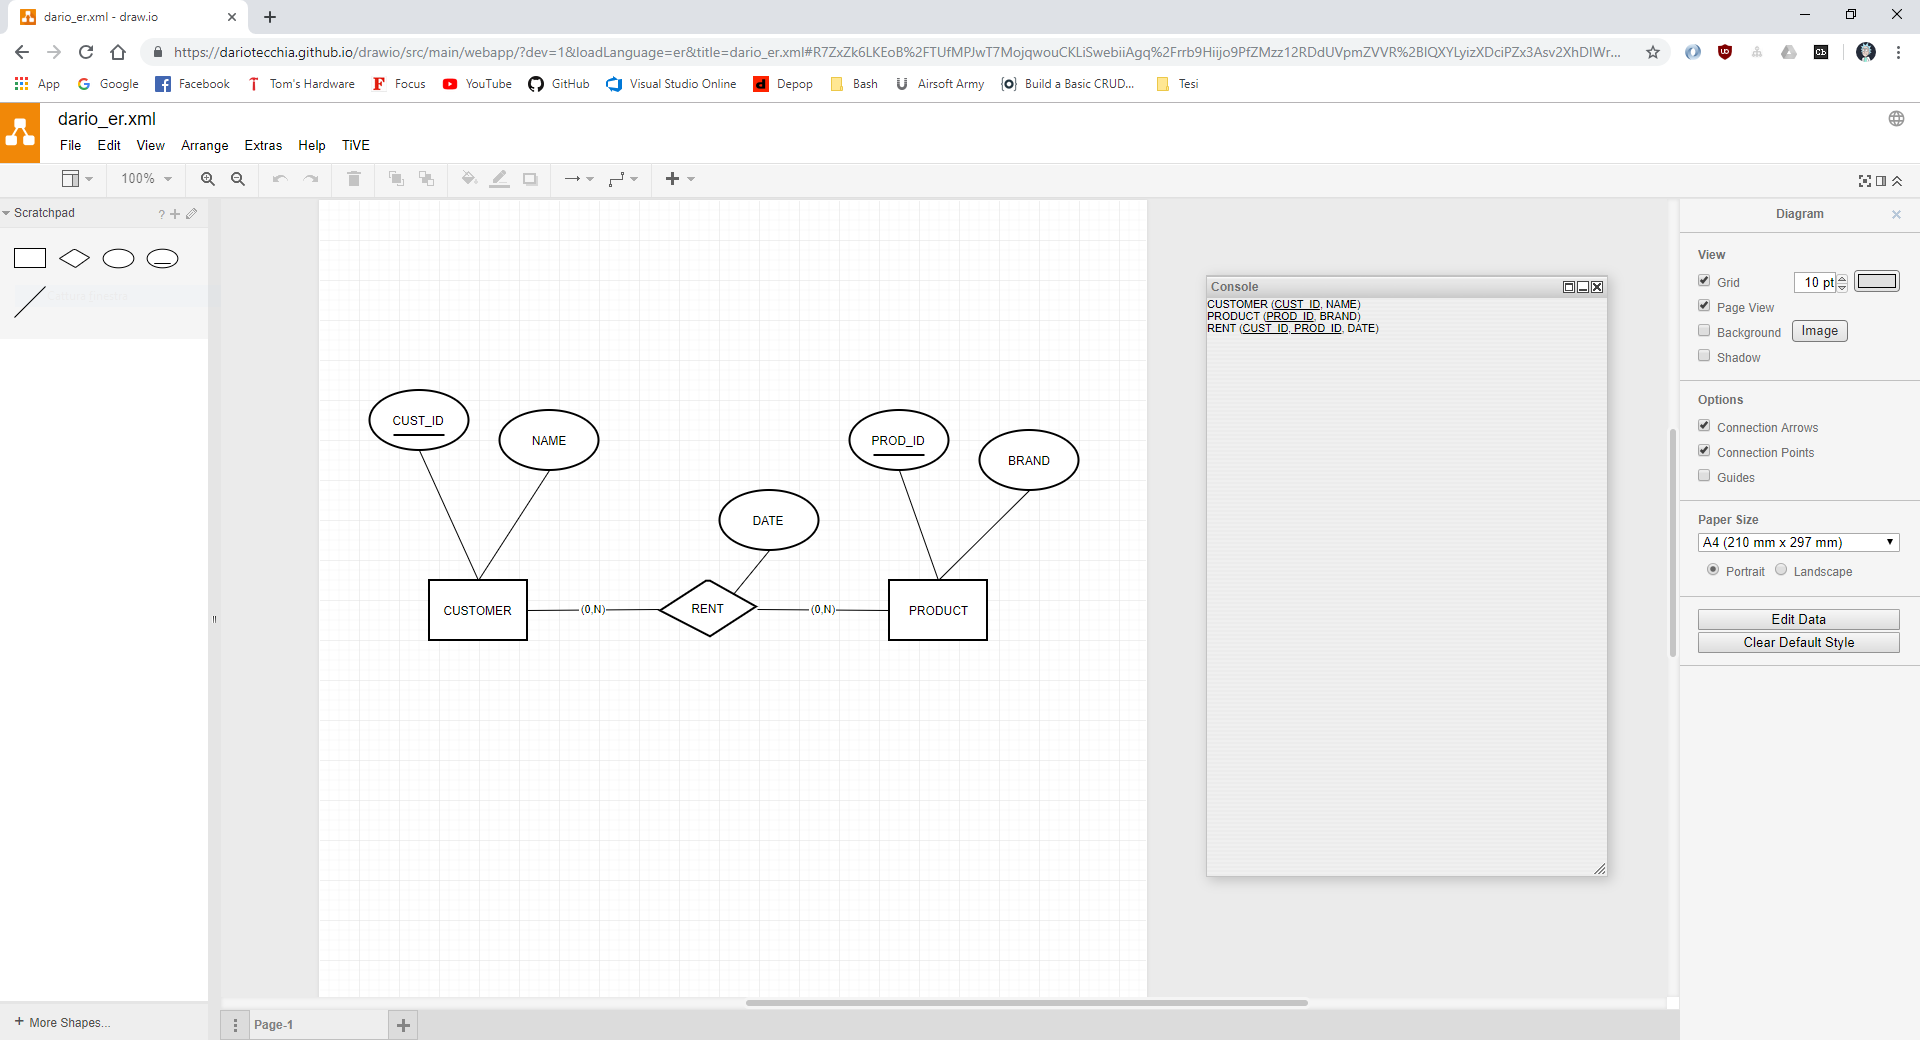
\includegraphics[scale=0.20]{Figure/semanticTranslation.PNG}
                    \caption{TiveJS con la traduzione semantica di un diagramma entità-relazione mostrata in una console (sulla destra)}
                    \label{fig:semanticTranslation}
                \end{figure}

                \begin{figure}[htbp]
                    \centering
                    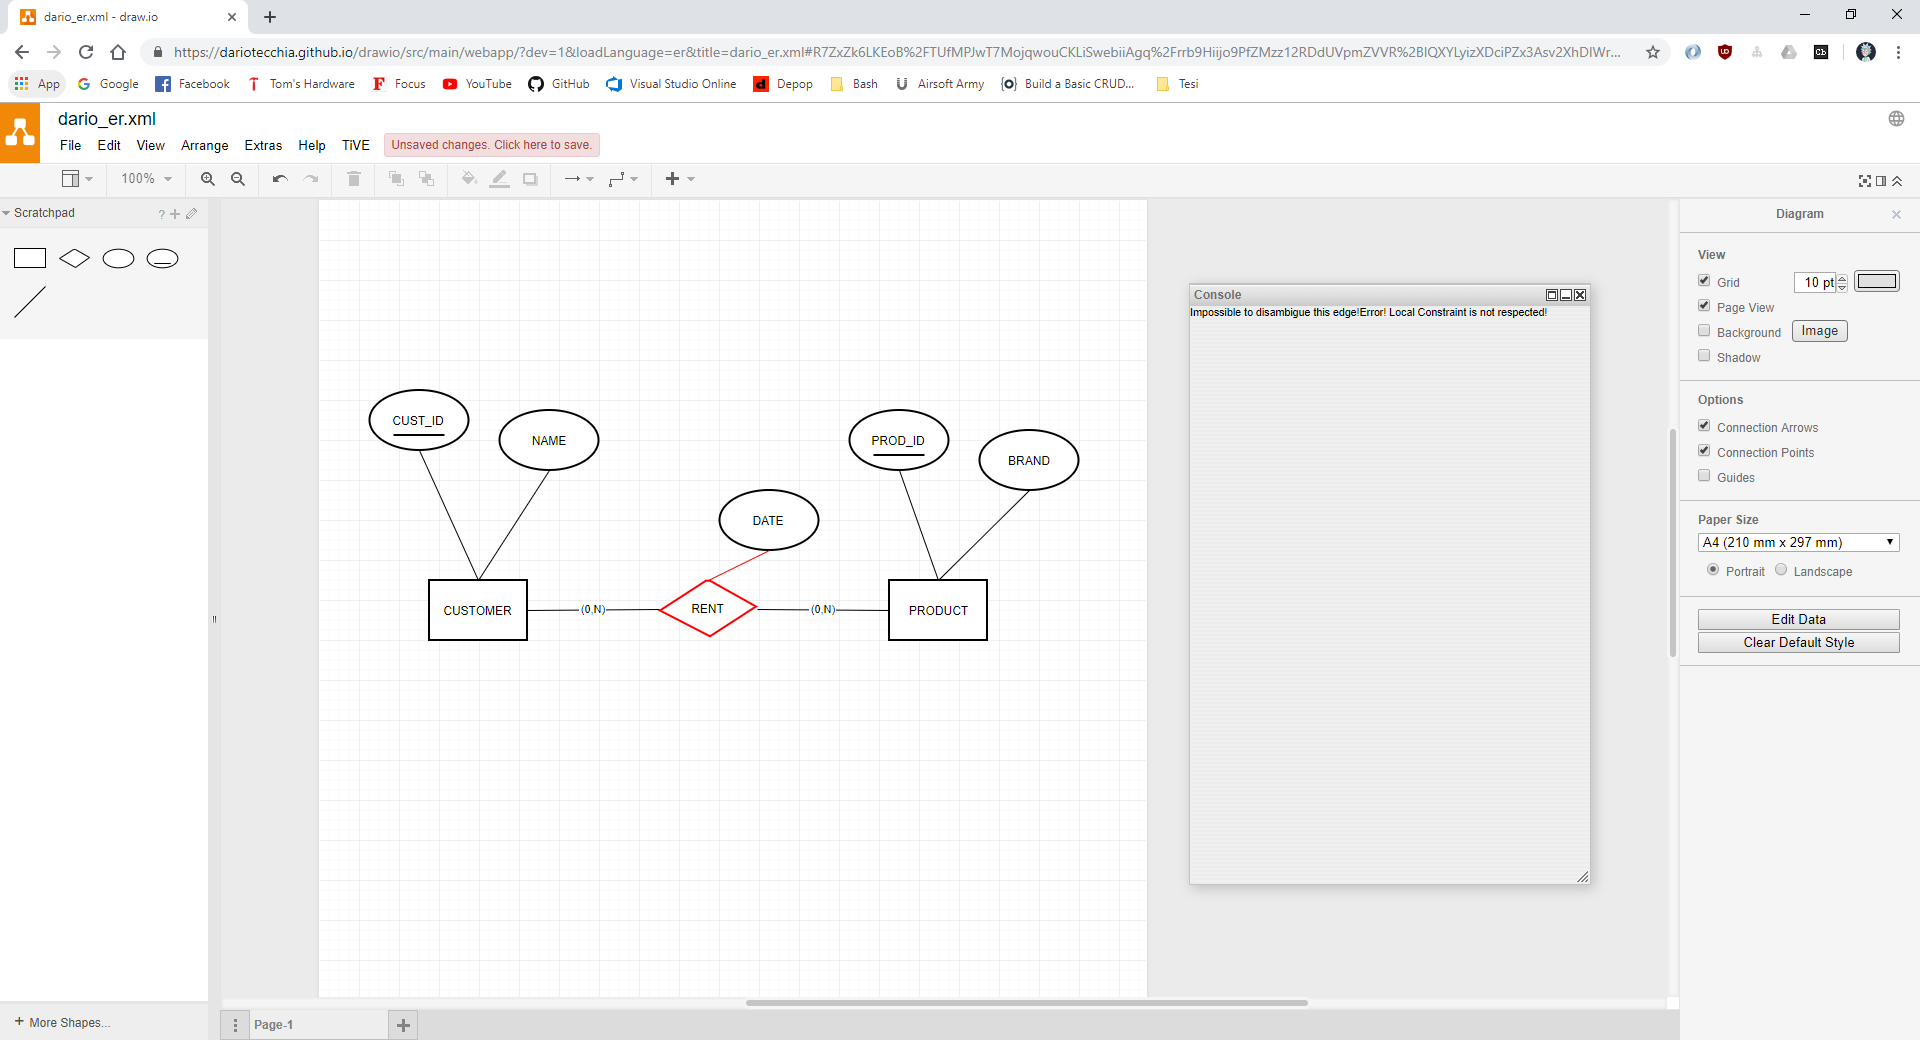
\includegraphics[scale=0.20]{Figure/semanticTranslation_error.PNG}
                    \caption{TiveJS con gli errori mostrati in una console (sulla destra)}
                    \label{fig:semanticTranslation_error}
                \end{figure}

    \section{Tecnologie Utilizzate: JavaScript}
        TiveJS è stata implementata completamente in JavaScript per far si che potesse girare su ogni browser web.
        JavaScript, a volte abbreviato con JS, è un linguaggio di programmazione interpretato ad alto livello. Standardizzato per la prima volta nel 1997 con il nome di ECMAScript (attualmente l'ultima release è ECMAScript 2018~\cite{ecmascript}), insieme all'HTML e il CSS è una delle tecnologie alla base del World Wide Web.
        In questa sezione esamino alcuni dei punti di forza di JavaScript, così da capire quali sono le sue particolarità.

        \subsection{Punti di Forza di JavaScript}

            \subsubsection{Ricco di librerie}
                JavaScript, oltre le sue librerie standard, conta un numero impressionante di librerie scritte da una community molto attiva. Dispone di API per lavorare con testo, matrici, date, espressioni regolari e DOM\footnote{Document Object Model}.

            \subsubsection{Supporto universale}
                Tutti i moderni browser web supportano nativamente JavaScript con gli interpreti implementati al loro interno.
            
            \subsubsection{Multi-paradigma}
                JavaScript è un linguaggio multi-paradigma, che supporta la programmazione basata sugli eventi, la programmazione funzionale e quella imperativa (inclusa la programmazione orientata agli ogetti).

            \subsubsection{Portabile}
                JavaScript è un linguaggio portabile. E' possibile usarlo su diverse piattaforme come: \textit{Linux, Windows, OSx, iOS e Android}. Questo è possibile perchè non dipende dalla macchina dove gira essendo interpretato e non compilato. E' necessario però un interprete JavaScript.

            \subsubsection{Semplice}
                Molto semplice da imparare e perfetto da usare come linguaggio accademico essendo un linguaggio ad alto livello.

            \subsubsection{Gratis}
                JavaScript è totalmente gratis ed è possibile utilizzarlo e distribuirlo senza restrizioni di copyright. Nonostante questo, alle spalle ha una community attivissima.

        \subsection{Principali Applicazioni}
            Pur essendo un linguaggio rilasciato per i browser web, Netscape, nel 1995 introdusse una nuova implementazione del linguaggio per lo scripting server-side. Una delle implementazioni server-side più famosa è Node.js.

        \section{Librerie utilizzate nel Progetto}
            \subsubsection{mxGraph}
                Come accennato, una delle librerie utilizzate all'interno di TiveJS è mxGraph. Serve per lo sviluppo di diagrammi e permette la creazione di applicazioni interattive per la creazione di grafi e diagrammi. Oltre che in JavaScript, la libreria è scritta anche in linguaggi server side quali PHP, .NET e Java~\cite{mxgraph}.
            \subsubsection{jQuery}
                jQuery risulta essere la libreria JavaScript più utilizzata su Internet per via della facilità di installazione e utilizzo.
                \newline
                Lo slogan di jQuery non a caso è \textit{<<write less, do more>>} poichè nasce con l'intenzione di semplificare la selezione, la manipolazione, la gestione degli eventi e l'animazione di elementi DOM in pagine HTML, nonchè implementare funzionalità AJAX~\cite{jquery}.
                \newline
                Fornisce agli sviluppatori un'interfaccia semplice, accessibile attraverso il caratteristico simbolo \textbf{\$}, astraendo comandi molto più complessi offerti da JavaScript. E' un software libero.

\chapter{Contesti d'utilizzo}
    \section{Entitiy Relationship}
    \section{Flowchart}
    \section{Tree}

\chapter{Conclusioni e Sviluppi Futuri}
    Riassumendo in questo lavoro ho presentato un sistema scritto interamente in JavaScript per il riconoscimento e la verifica di linguaggi diagrammatici in grado di permettere lo sviluppo di una sentenza visiva e di ottenere, applicando delle definizioni, una traduzione semantica di quest'ultima.
    \newline
    In tutta la tesi ho analizzato vari casi d'utilizzo, uno in cui l'applicazione delle definizioni va a buon fine ed uno in cui non va a buon fine. Ho presentato i dettagli implementativi di TiveJS illustrando le parti di codice di maggior interesse.
    \newline
    In futuro l'applicazione verrà integrata con l'ecosistema LoCoMoTiVE permettendo di creare un'unica applicazione dove il progettista può creare delle definizioni e testarle direttamente all'interno di quest'ultima.

% ********************************** Appendices ********************************

% ********************************** Appendices ********************************

\begin{appendices} % Using appendices environment for more functionality

    \chapter{Codici}
    \begin{spacing}{0.5}
        \lstinputlisting[language=JavaScript, caption={\textbf{Specifica di un linguaggio in formato XML, in questo caso quello per Albero Binario}}, label={appendix:xml_definition}, language=Xml]{SourceCode/tree_specific.xml}
        \newpage
        \lstinputlisting[language=JavaScript, basicstyle=\scriptsize, caption={\textbf{Specifica sintattica di un Albero}}, label={appendix:jsonDefinition}, language=Xml]{SourceCode/newDefinition.json}
        \newpage
        \lstinputlisting[language=JavaScript, caption={\textbf{Specifica semantica di un linguaggio in formato JSON, in questo caso quello per Albero}}, label={appendix:jsonSemanticDefinition}, language=Xml]{SourceCode/newSemanticDefinition.json}
    \end{spacing}
    \begin{spacing}{0.7}
        \newpage
        \lstinputlisting[language=JavaScript, basicstyle=\tiny, caption={\textbf{Specifica semantica di un linguaggio in formato JSON, in questo caso quello per FlowChart}}, label={appendix:ERjsonSemanticDefinition}, language=Xml]{SourceCode/EXAMPLES/flowchartp/newSemanticDefinition.json}
    \end{spacing}
    
\end{appendices}

% ********************************** Back Matter *******************************
% Backmatter should be commented out, if you are using appendices after References
%\backmatter

% ********************************** Bibliography ******************************
\begin{spacing}{0.9}

% To use the conventional natbib style referencing
% Bibliography style previews: http://nodonn.tipido.net/bibstyle.php
% Reference styles: http://sites.stat.psu.edu/~surajit/present/bib.htm

% \bibliographystyle{apalike}
%\bibliographystyle{plain}
%\bibliographystyle{unsrt} % Use for unsorted references  
\bibliographystyle{plainnat} % use this to have URLs listed in References
\cleardoublepage
\bibliography{References/references} % Path to your References.bib file


% If you would like to use BibLaTeX for your references, pass `custombib' as
% an option in the document class. The location of 'reference.bib' should be
% specified in the preamble.tex file in the custombib section.
% Comment out the lines related to natbib above and uncomment the following line.

%\printbibliography[heading=bibintoc, title={References}]


\end{spacing}


% *************************************** Index ********************************
\printthesisindex % If index is present

\end{document}

